% Created by tikzDevice version 0.12 on 2019-02-08 07:26:39
% !TEX encoding = UTF-8 Unicode
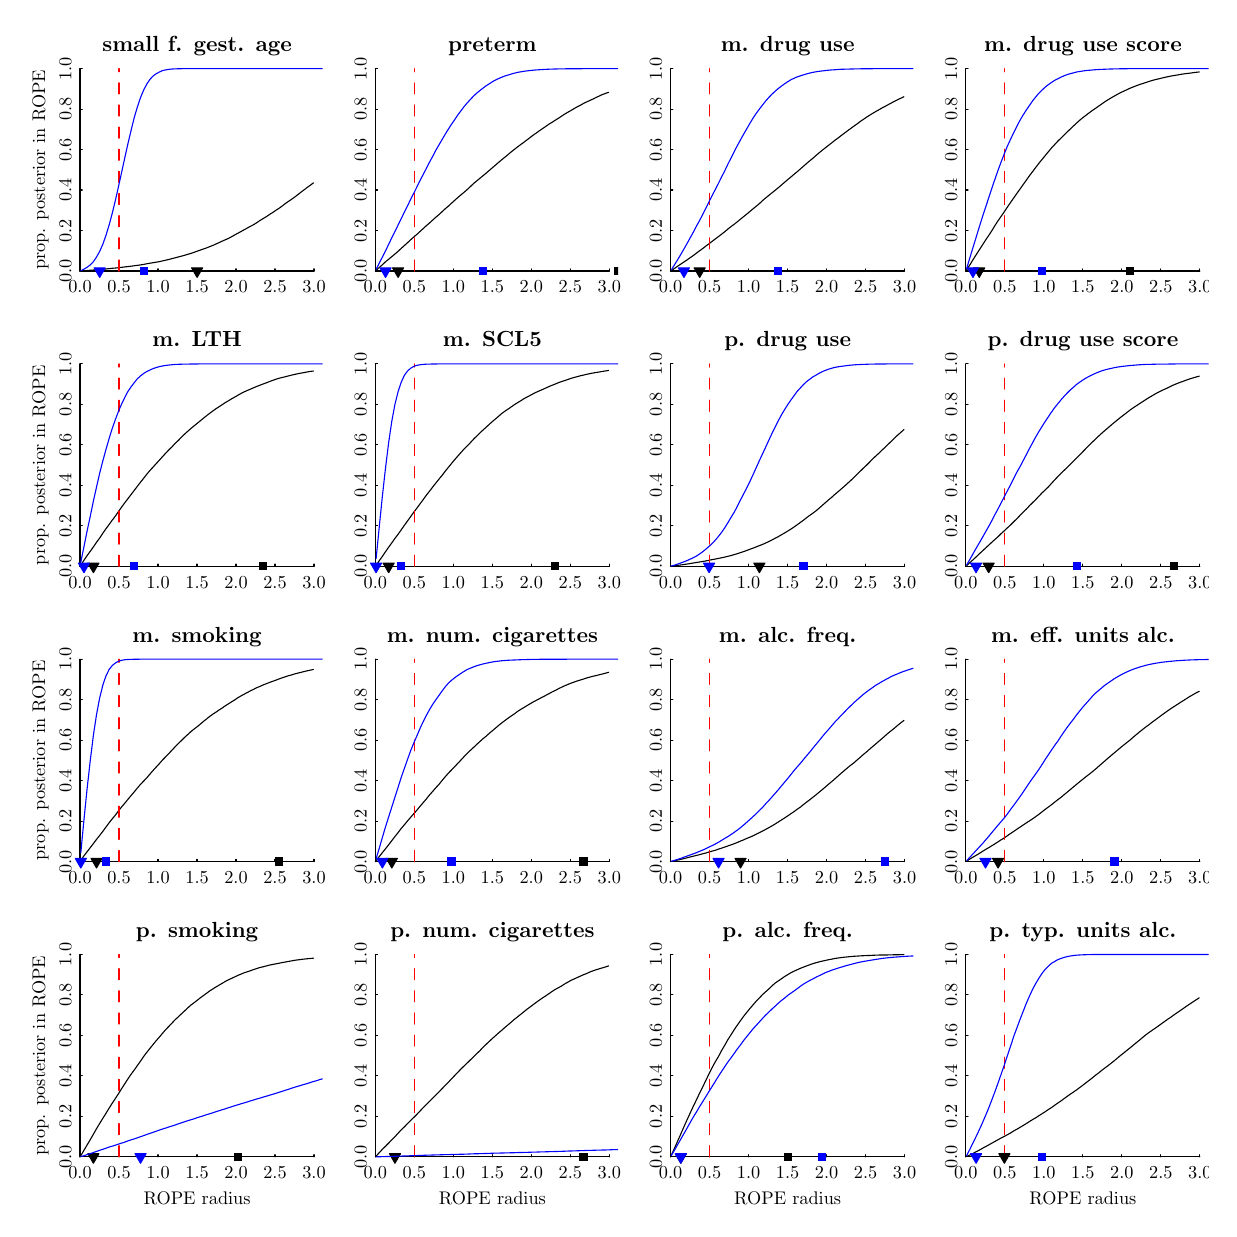
\begin{tikzpicture}[x=1pt,y=1pt]
\definecolor{fillColor}{RGB}{255,255,255}
\path[use as bounding box,fill=fillColor,fill opacity=0.00] (0,0) rectangle (426.79,426.79);
\begin{scope}
\path[clip] ( 15.84,335.93) rectangle (106.62,414.91);
\definecolor{drawColor}{RGB}{0,0,0}

\path[draw=drawColor,line width= 0.4pt,line join=round,line cap=round] ( 19.20,338.87) --
	( 20.34,338.94) --
	( 21.47,339.02) --
	( 22.61,339.13) --
	( 23.75,339.21) --
	( 24.88,339.31) --
	( 26.02,339.40) --
	( 27.15,339.50) --
	( 28.29,339.59) --
	( 29.42,339.72) --
	( 30.56,339.84) --
	( 31.70,339.93) --
	( 32.83,340.05) --
	( 33.97,340.19) --
	( 35.10,340.34) --
	( 36.24,340.46) --
	( 37.38,340.60) --
	( 38.51,340.76) --
	( 39.65,340.90) --
	( 40.78,341.06) --
	( 41.92,341.25) --
	( 43.06,341.48) --
	( 44.19,341.67) --
	( 45.33,341.87) --
	( 46.46,342.05) --
	( 47.60,342.24) --
	( 48.73,342.51) --
	( 49.87,342.77) --
	( 51.01,343.03) --
	( 52.14,343.33) --
	( 53.28,343.63) --
	( 54.41,343.92) --
	( 55.55,344.22) --
	( 56.69,344.54) --
	( 57.82,344.88) --
	( 58.96,345.21) --
	( 60.09,345.59) --
	( 61.23,346.01) --
	( 62.37,346.42) --
	( 63.50,346.81) --
	( 64.64,347.21) --
	( 65.77,347.66) --
	( 66.91,348.11) --
	( 68.04,348.61) --
	( 69.18,349.13) --
	( 70.32,349.66) --
	( 71.45,350.16) --
	( 72.59,350.65) --
	( 73.72,351.27) --
	( 74.86,351.92) --
	( 76.00,352.53) --
	( 77.13,353.14) --
	( 78.27,353.79) --
	( 79.40,354.40) --
	( 80.54,355.04) --
	( 81.67,355.61) --
	( 82.81,356.34) --
	( 83.95,357.11) --
	( 85.08,357.79) --
	( 86.22,358.48) --
	( 87.35,359.25) --
	( 88.49,359.97) --
	( 89.63,360.75) --
	( 90.76,361.46) --
	( 91.90,362.29) --
	( 93.03,363.18) --
	( 94.17,363.98) --
	( 95.31,364.74) --
	( 96.44,365.53) --
	( 97.58,366.41) --
	( 98.71,367.30) --
	( 99.85,368.16) --
	(100.98,369.03) --
	(102.12,369.85) --
	(103.26,370.71);
\end{scope}
\begin{scope}
\path[clip] (  0.00,320.09) rectangle (106.70,426.79);
\definecolor{drawColor}{RGB}{0,0,0}

\node[text=drawColor,rotate= 90.00,anchor=base,inner sep=0pt, outer sep=0pt, scale=  0.66] at (  6.34,375.42) {prop. posterior in ROPE};

\node[text=drawColor,anchor=base,inner sep=0pt, outer sep=0pt, scale=  0.79] at ( 61.23,418.12) {\bfseries small f. gest. age};
\end{scope}
\begin{scope}
\path[clip] (  0.00,  0.00) rectangle (426.79,426.79);
\definecolor{drawColor}{RGB}{0,0,0}

\path[draw=drawColor,line width= 0.4pt,line join=round,line cap=round] ( 18.92,338.86) -- (103.47,338.86);

\path[draw=drawColor,line width= 0.4pt,line join=round,line cap=round] ( 18.92,338.86) -- ( 18.92,339.65);

\path[draw=drawColor,line width= 0.4pt,line join=round,line cap=round] ( 33.01,338.86) -- ( 33.01,339.65);

\path[draw=drawColor,line width= 0.4pt,line join=round,line cap=round] ( 47.10,338.86) -- ( 47.10,339.65);

\path[draw=drawColor,line width= 0.4pt,line join=round,line cap=round] ( 61.20,338.86) -- ( 61.20,339.65);

\path[draw=drawColor,line width= 0.4pt,line join=round,line cap=round] ( 75.29,338.86) -- ( 75.29,339.65);

\path[draw=drawColor,line width= 0.4pt,line join=round,line cap=round] ( 89.38,338.86) -- ( 89.38,339.65);

\path[draw=drawColor,line width= 0.4pt,line join=round,line cap=round] (103.47,338.86) -- (103.47,339.65);

\node[text=drawColor,anchor=base,inner sep=0pt, outer sep=0pt, scale=  0.66] at ( 18.92,330.94) {0.0};

\node[text=drawColor,anchor=base,inner sep=0pt, outer sep=0pt, scale=  0.66] at ( 33.01,330.94) {0.5};

\node[text=drawColor,anchor=base,inner sep=0pt, outer sep=0pt, scale=  0.66] at ( 47.10,330.94) {1.0};

\node[text=drawColor,anchor=base,inner sep=0pt, outer sep=0pt, scale=  0.66] at ( 61.20,330.94) {1.5};

\node[text=drawColor,anchor=base,inner sep=0pt, outer sep=0pt, scale=  0.66] at ( 75.29,330.94) {2.0};

\node[text=drawColor,anchor=base,inner sep=0pt, outer sep=0pt, scale=  0.66] at ( 89.38,330.94) {2.5};

\node[text=drawColor,anchor=base,inner sep=0pt, outer sep=0pt, scale=  0.66] at (103.47,330.94) {3.0};

\path[draw=drawColor,line width= 0.4pt,line join=round,line cap=round] ( 18.92,338.86) -- ( 18.92,411.99);

\path[draw=drawColor,line width= 0.4pt,line join=round,line cap=round] ( 18.92,338.86) -- ( 19.71,338.86);

\path[draw=drawColor,line width= 0.4pt,line join=round,line cap=round] ( 18.92,353.48) -- ( 19.71,353.48);

\path[draw=drawColor,line width= 0.4pt,line join=round,line cap=round] ( 18.92,368.11) -- ( 19.71,368.11);

\path[draw=drawColor,line width= 0.4pt,line join=round,line cap=round] ( 18.92,382.74) -- ( 19.71,382.74);

\path[draw=drawColor,line width= 0.4pt,line join=round,line cap=round] ( 18.92,397.36) -- ( 19.71,397.36);

\path[draw=drawColor,line width= 0.4pt,line join=round,line cap=round] ( 18.92,411.99) -- ( 19.71,411.99);

\node[text=drawColor,rotate= 90.00,anchor=base,inner sep=0pt, outer sep=0pt, scale=  0.66] at ( 15.75,338.86) {0.0};

\node[text=drawColor,rotate= 90.00,anchor=base,inner sep=0pt, outer sep=0pt, scale=  0.66] at ( 15.75,353.48) {0.2};

\node[text=drawColor,rotate= 90.00,anchor=base,inner sep=0pt, outer sep=0pt, scale=  0.66] at ( 15.75,368.11) {0.4};

\node[text=drawColor,rotate= 90.00,anchor=base,inner sep=0pt, outer sep=0pt, scale=  0.66] at ( 15.75,382.74) {0.6};

\node[text=drawColor,rotate= 90.00,anchor=base,inner sep=0pt, outer sep=0pt, scale=  0.66] at ( 15.75,397.36) {0.8};

\node[text=drawColor,rotate= 90.00,anchor=base,inner sep=0pt, outer sep=0pt, scale=  0.66] at ( 15.75,411.99) {1.0};
\end{scope}
\begin{scope}
\path[clip] ( 15.84,335.93) rectangle (106.62,414.91);
\definecolor{drawColor}{RGB}{0,0,0}

\path[draw=drawColor,line width= 0.4pt,line join=round,line cap=round] (131.65,338.86) --
	(131.65,411.99);
\definecolor{drawColor}{RGB}{255,0,0}

\path[draw=drawColor,line width= 0.4pt,dash pattern=on 4pt off 4pt ,line join=round,line cap=round] ( 33.01,338.86) --
	( 33.01,411.99);
\definecolor{fillColor}{RGB}{0,0,0}

\path[fill=fillColor] (130.17,337.37) --
	(133.14,337.37) --
	(133.14,340.34) --
	(130.17,340.34) --
	cycle;
\definecolor{drawColor}{RGB}{0,0,0}

\path[draw=drawColor,line width= 0.4pt,line join=round,line cap=round,fill=fillColor] ( 61.23,336.55) --
	( 63.23,340.01) --
	( 59.23,340.01) --
	cycle;
\definecolor{drawColor}{RGB}{0,0,255}

\path[draw=drawColor,line width= 0.4pt,line join=round,line cap=round] ( 19.20,338.95) --
	( 20.34,339.52) --
	( 21.47,340.21) --
	( 22.61,341.07) --
	( 23.75,342.24) --
	( 24.88,343.90) --
	( 26.02,345.96) --
	( 27.15,348.51) --
	( 28.29,351.73) --
	( 29.42,355.45) --
	( 30.56,359.70) --
	( 31.70,364.40) --
	( 32.83,369.43) --
	( 33.97,374.60) --
	( 35.10,379.80) --
	( 36.24,384.92) --
	( 37.38,389.72) --
	( 38.51,394.31) --
	( 39.65,398.16) --
	( 40.78,401.51) --
	( 41.92,404.26) --
	( 43.06,406.44) --
	( 44.19,408.12) --
	( 45.33,409.33) --
	( 46.46,410.16) --
	( 47.60,410.76) --
	( 48.73,411.28) --
	( 49.87,411.52) --
	( 51.01,411.72) --
	( 52.14,411.84) --
	( 53.28,411.90) --
	( 54.41,411.94) --
	( 55.55,411.96) --
	( 56.69,411.97) --
	( 57.82,411.98) --
	( 58.96,411.99) --
	( 60.09,411.99) --
	( 61.23,411.99) --
	( 62.37,411.99) --
	( 63.50,411.99) --
	( 64.64,411.99) --
	( 65.77,411.99) --
	( 66.91,411.99) --
	( 68.04,411.99) --
	( 69.18,411.99) --
	( 70.32,411.99) --
	( 71.45,411.99) --
	( 72.59,411.99) --
	( 73.72,411.99) --
	( 74.86,411.99) --
	( 76.00,411.99) --
	( 77.13,411.99) --
	( 78.27,411.99) --
	( 79.40,411.99) --
	( 80.54,411.99) --
	( 81.67,411.99) --
	( 82.81,411.99) --
	( 83.95,411.99) --
	( 85.08,411.99) --
	( 86.22,411.99) --
	( 87.35,411.99) --
	( 88.49,411.99) --
	( 89.63,411.99) --
	( 90.76,411.99) --
	( 91.90,411.99) --
	( 93.03,411.99) --
	( 94.17,411.99) --
	( 95.31,411.99) --
	( 96.44,411.99) --
	( 97.58,411.99) --
	( 98.71,411.99) --
	( 99.85,411.99) --
	(100.98,411.99) --
	(102.12,411.99) --
	(103.26,411.99) --
	(104.39,411.99) --
	(105.53,411.99) --
	(106.66,411.99) --
	(107.80,411.99) --
	(108.94,411.99) --
	(110.07,411.99) --
	(111.21,411.99) --
	(112.34,411.99) --
	(113.48,411.99) --
	(114.62,411.99) --
	(115.75,411.99) --
	(116.89,411.99) --
	(118.02,411.99) --
	(119.16,411.99) --
	(120.29,411.99) --
	(121.43,411.99) --
	(122.57,411.99) --
	(123.70,411.99) --
	(124.84,411.99) --
	(125.97,411.99) --
	(127.11,411.99) --
	(128.25,411.99) --
	(129.38,411.99) --
	(130.52,411.99) --
	(131.65,411.99);
\definecolor{fillColor}{RGB}{0,0,255}

\path[fill=fillColor] ( 40.43,337.37) --
	( 43.40,337.37) --
	( 43.40,340.34) --
	( 40.43,340.34) --
	cycle;

\path[draw=drawColor,line width= 0.4pt,line join=round,line cap=round,fill=fillColor] ( 26.02,336.55) --
	( 28.02,340.01) --
	( 24.02,340.01) --
	cycle;
\end{scope}
\begin{scope}
\path[clip] (122.54,335.93) rectangle (213.32,414.91);
\definecolor{drawColor}{RGB}{0,0,0}

\path[draw=drawColor,line width= 0.4pt,line join=round,line cap=round] (125.90,339.10) --
	(127.04,340.10) --
	(128.17,341.11) --
	(129.31,342.20) --
	(130.44,343.10) --
	(131.58,344.06) --
	(132.72,345.01) --
	(133.85,345.97) --
	(134.99,347.04) --
	(136.12,348.06) --
	(137.26,349.08) --
	(138.39,350.15) --
	(139.53,351.16) --
	(140.67,352.12) --
	(141.80,353.16) --
	(142.94,354.20) --
	(144.07,355.24) --
	(145.21,356.22) --
	(146.35,357.26) --
	(147.48,358.29) --
	(148.62,359.24) --
	(149.75,360.29) --
	(150.89,361.35) --
	(152.02,362.30) --
	(153.16,363.37) --
	(154.30,364.39) --
	(155.43,365.40) --
	(156.57,366.38) --
	(157.70,367.30) --
	(158.84,368.30) --
	(159.98,369.37) --
	(161.11,370.46) --
	(162.25,371.40) --
	(163.38,372.34) --
	(164.52,373.27) --
	(165.66,374.22) --
	(166.79,375.19) --
	(167.93,376.19) --
	(169.06,377.13) --
	(170.20,378.14) --
	(171.33,379.08) --
	(172.47,380.01) --
	(173.61,380.95) --
	(174.74,381.92) --
	(175.88,382.81) --
	(177.01,383.70) --
	(178.15,384.54) --
	(179.29,385.37) --
	(180.42,386.22) --
	(181.56,387.11) --
	(182.69,387.96) --
	(183.83,388.76) --
	(184.97,389.57) --
	(186.10,390.36) --
	(187.24,391.13) --
	(188.37,391.92) --
	(189.51,392.61) --
	(190.64,393.34) --
	(191.78,394.06) --
	(192.92,394.80) --
	(194.05,395.55) --
	(195.19,396.23) --
	(196.32,396.86) --
	(197.46,397.54) --
	(198.60,398.20) --
	(199.73,398.77) --
	(200.87,399.42) --
	(202.00,399.96) --
	(203.14,400.47) --
	(204.27,401.00) --
	(205.41,401.58) --
	(206.55,402.09) --
	(207.68,402.62) --
	(208.82,403.04) --
	(209.95,403.44);
\end{scope}
\begin{scope}
\path[clip] (106.70,320.09) rectangle (213.40,426.79);
\definecolor{drawColor}{RGB}{0,0,0}

\node[text=drawColor,anchor=base,inner sep=0pt, outer sep=0pt, scale=  0.79] at (167.93,418.12) {\bfseries preterm};
\end{scope}
\begin{scope}
\path[clip] (  0.00,  0.00) rectangle (426.79,426.79);
\definecolor{drawColor}{RGB}{0,0,0}

\path[draw=drawColor,line width= 0.4pt,line join=round,line cap=round] (125.62,338.86) -- (210.17,338.86);

\path[draw=drawColor,line width= 0.4pt,line join=round,line cap=round] (125.62,338.86) -- (125.62,339.65);

\path[draw=drawColor,line width= 0.4pt,line join=round,line cap=round] (139.71,338.86) -- (139.71,339.65);

\path[draw=drawColor,line width= 0.4pt,line join=round,line cap=round] (153.80,338.86) -- (153.80,339.65);

\path[draw=drawColor,line width= 0.4pt,line join=round,line cap=round] (167.89,338.86) -- (167.89,339.65);

\path[draw=drawColor,line width= 0.4pt,line join=round,line cap=round] (181.98,338.86) -- (181.98,339.65);

\path[draw=drawColor,line width= 0.4pt,line join=round,line cap=round] (196.08,338.86) -- (196.08,339.65);

\path[draw=drawColor,line width= 0.4pt,line join=round,line cap=round] (210.17,338.86) -- (210.17,339.65);

\node[text=drawColor,anchor=base,inner sep=0pt, outer sep=0pt, scale=  0.66] at (125.62,330.94) {0.0};

\node[text=drawColor,anchor=base,inner sep=0pt, outer sep=0pt, scale=  0.66] at (139.71,330.94) {0.5};

\node[text=drawColor,anchor=base,inner sep=0pt, outer sep=0pt, scale=  0.66] at (153.80,330.94) {1.0};

\node[text=drawColor,anchor=base,inner sep=0pt, outer sep=0pt, scale=  0.66] at (167.89,330.94) {1.5};

\node[text=drawColor,anchor=base,inner sep=0pt, outer sep=0pt, scale=  0.66] at (181.98,330.94) {2.0};

\node[text=drawColor,anchor=base,inner sep=0pt, outer sep=0pt, scale=  0.66] at (196.08,330.94) {2.5};

\node[text=drawColor,anchor=base,inner sep=0pt, outer sep=0pt, scale=  0.66] at (210.17,330.94) {3.0};

\path[draw=drawColor,line width= 0.4pt,line join=round,line cap=round] (125.62,338.86) -- (125.62,411.99);

\path[draw=drawColor,line width= 0.4pt,line join=round,line cap=round] (125.62,338.86) -- (126.41,338.86);

\path[draw=drawColor,line width= 0.4pt,line join=round,line cap=round] (125.62,353.48) -- (126.41,353.48);

\path[draw=drawColor,line width= 0.4pt,line join=round,line cap=round] (125.62,368.11) -- (126.41,368.11);

\path[draw=drawColor,line width= 0.4pt,line join=round,line cap=round] (125.62,382.74) -- (126.41,382.74);

\path[draw=drawColor,line width= 0.4pt,line join=round,line cap=round] (125.62,397.36) -- (126.41,397.36);

\path[draw=drawColor,line width= 0.4pt,line join=round,line cap=round] (125.62,411.99) -- (126.41,411.99);

\node[text=drawColor,rotate= 90.00,anchor=base,inner sep=0pt, outer sep=0pt, scale=  0.66] at (122.45,338.86) {0.0};

\node[text=drawColor,rotate= 90.00,anchor=base,inner sep=0pt, outer sep=0pt, scale=  0.66] at (122.45,353.48) {0.2};

\node[text=drawColor,rotate= 90.00,anchor=base,inner sep=0pt, outer sep=0pt, scale=  0.66] at (122.45,368.11) {0.4};

\node[text=drawColor,rotate= 90.00,anchor=base,inner sep=0pt, outer sep=0pt, scale=  0.66] at (122.45,382.74) {0.6};

\node[text=drawColor,rotate= 90.00,anchor=base,inner sep=0pt, outer sep=0pt, scale=  0.66] at (122.45,397.36) {0.8};

\node[text=drawColor,rotate= 90.00,anchor=base,inner sep=0pt, outer sep=0pt, scale=  0.66] at (122.45,411.99) {1.0};
\end{scope}
\begin{scope}
\path[clip] (122.54,335.93) rectangle (213.32,414.91);
\definecolor{drawColor}{RGB}{0,0,0}

\path[draw=drawColor,line width= 0.4pt,line join=round,line cap=round] (238.35,338.86) --
	(238.35,411.99);
\definecolor{drawColor}{RGB}{255,0,0}

\path[draw=drawColor,line width= 0.4pt,dash pattern=on 4pt off 4pt ,line join=round,line cap=round] (139.71,338.86) --
	(139.71,411.99);
\definecolor{fillColor}{RGB}{0,0,0}

\path[fill=fillColor] (211.88,337.37) --
	(214.85,337.37) --
	(214.85,340.34) --
	(211.88,340.34) --
	cycle;
\definecolor{drawColor}{RGB}{0,0,0}

\path[draw=drawColor,line width= 0.4pt,line join=round,line cap=round,fill=fillColor] (133.85,336.55) --
	(135.85,340.01) --
	(131.85,340.01) --
	cycle;
\definecolor{drawColor}{RGB}{0,0,255}

\path[draw=drawColor,line width= 0.4pt,line join=round,line cap=round] (125.90,339.47) --
	(127.04,341.72) --
	(128.17,343.91) --
	(129.31,346.13) --
	(130.44,348.51) --
	(131.58,350.86) --
	(132.72,353.14) --
	(133.85,355.47) --
	(134.99,357.81) --
	(136.12,360.12) --
	(137.26,362.41) --
	(138.39,364.78) --
	(139.53,366.99) --
	(140.67,369.29) --
	(141.80,371.59) --
	(142.94,373.79) --
	(144.07,375.96) --
	(145.21,378.19) --
	(146.35,380.29) --
	(147.48,382.47) --
	(148.62,384.43) --
	(149.75,386.36) --
	(150.89,388.31) --
	(152.02,390.13) --
	(153.16,391.91) --
	(154.30,393.55) --
	(155.43,395.25) --
	(156.57,396.76) --
	(157.70,398.27) --
	(158.84,399.61) --
	(159.98,400.85) --
	(161.11,402.06) --
	(162.25,403.12) --
	(163.38,404.04) --
	(164.52,404.92) --
	(165.66,405.80) --
	(166.79,406.49) --
	(167.93,407.25) --
	(169.06,407.88) --
	(170.20,408.42) --
	(171.33,408.90) --
	(172.47,409.33) --
	(173.61,409.67) --
	(174.74,410.04) --
	(175.88,410.35) --
	(177.01,410.63) --
	(178.15,410.83) --
	(179.29,411.02) --
	(180.42,411.17) --
	(181.56,411.30) --
	(182.69,411.42) --
	(183.83,411.52) --
	(184.97,411.60) --
	(186.10,411.66) --
	(187.24,411.73) --
	(188.37,411.78) --
	(189.51,411.82) --
	(190.64,411.85) --
	(191.78,411.88) --
	(192.92,411.89) --
	(194.05,411.92) --
	(195.19,411.93) --
	(196.32,411.93) --
	(197.46,411.94) --
	(198.60,411.95) --
	(199.73,411.95) --
	(200.87,411.97) --
	(202.00,411.97) --
	(203.14,411.98) --
	(204.27,411.98) --
	(205.41,411.98) --
	(206.55,411.98) --
	(207.68,411.98) --
	(208.82,411.98) --
	(209.95,411.98) --
	(211.09,411.98) --
	(212.23,411.98) --
	(213.36,411.98) --
	(214.50,411.98) --
	(215.63,411.98) --
	(216.77,411.98) --
	(217.91,411.99) --
	(219.04,411.99) --
	(220.18,411.99) --
	(221.31,411.99) --
	(222.45,411.99) --
	(223.58,411.99) --
	(224.72,411.99) --
	(225.86,411.99) --
	(226.99,411.99) --
	(228.13,411.99) --
	(229.26,411.99) --
	(230.40,411.99) --
	(231.54,411.99) --
	(232.67,411.99) --
	(233.81,411.99) --
	(234.94,411.99) --
	(236.08,411.99) --
	(237.22,411.99) --
	(238.35,411.99);
\definecolor{fillColor}{RGB}{0,0,255}

\path[fill=fillColor] (163.03,337.37) --
	(166.00,337.37) --
	(166.00,340.34) --
	(163.03,340.34) --
	cycle;

\path[draw=drawColor,line width= 0.4pt,line join=round,line cap=round,fill=fillColor] (129.31,336.55) --
	(131.31,340.01) --
	(127.31,340.01) --
	cycle;
\end{scope}
\begin{scope}
\path[clip] (229.24,335.93) rectangle (320.01,414.91);
\definecolor{drawColor}{RGB}{0,0,0}

\path[draw=drawColor,line width= 0.4pt,line join=round,line cap=round] (232.60,339.00) --
	(233.73,339.79) --
	(234.87,340.60) --
	(236.01,341.36) --
	(237.14,342.11) --
	(238.28,342.88) --
	(239.41,343.68) --
	(240.55,344.47) --
	(241.68,345.33) --
	(242.82,346.20) --
	(243.96,346.99) --
	(245.09,347.89) --
	(246.23,348.72) --
	(247.36,349.60) --
	(248.50,350.46) --
	(249.64,351.32) --
	(250.77,352.18) --
	(251.91,353.06) --
	(253.04,354.04) --
	(254.18,354.93) --
	(255.32,355.77) --
	(256.45,356.66) --
	(257.59,357.61) --
	(258.72,358.52) --
	(259.86,359.44) --
	(260.99,360.39) --
	(262.13,361.34) --
	(263.27,362.27) --
	(264.40,363.21) --
	(265.54,364.30) --
	(266.67,365.26) --
	(267.81,366.18) --
	(268.95,367.10) --
	(270.08,368.01) --
	(271.22,368.94) --
	(272.35,369.90) --
	(273.49,370.89) --
	(274.62,371.87) --
	(275.76,372.79) --
	(276.90,373.79) --
	(278.03,374.71) --
	(279.17,375.69) --
	(280.30,376.69) --
	(281.44,377.69) --
	(282.58,378.66) --
	(283.71,379.57) --
	(284.85,380.59) --
	(285.98,381.55) --
	(287.12,382.50) --
	(288.26,383.39) --
	(289.39,384.28) --
	(290.53,385.16) --
	(291.66,386.07) --
	(292.80,386.90) --
	(293.93,387.77) --
	(295.07,388.63) --
	(296.21,389.49) --
	(297.34,390.31) --
	(298.48,391.15) --
	(299.61,391.95) --
	(300.75,392.81) --
	(301.89,393.59) --
	(303.02,394.37) --
	(304.16,395.10) --
	(305.29,395.80) --
	(306.43,396.48) --
	(307.57,397.10) --
	(308.70,397.76) --
	(309.84,398.35) --
	(310.97,398.98) --
	(312.11,399.59) --
	(313.24,400.18) --
	(314.38,400.78) --
	(315.52,401.30) --
	(316.65,401.85);
\end{scope}
\begin{scope}
\path[clip] (213.40,320.09) rectangle (320.09,426.79);
\definecolor{drawColor}{RGB}{0,0,0}

\node[text=drawColor,anchor=base,inner sep=0pt, outer sep=0pt, scale=  0.79] at (274.62,418.12) {\bfseries m. drug use};
\end{scope}
\begin{scope}
\path[clip] (  0.00,  0.00) rectangle (426.79,426.79);
\definecolor{drawColor}{RGB}{0,0,0}

\path[draw=drawColor,line width= 0.4pt,line join=round,line cap=round] (232.32,338.86) -- (316.87,338.86);

\path[draw=drawColor,line width= 0.4pt,line join=round,line cap=round] (232.32,338.86) -- (232.32,339.65);

\path[draw=drawColor,line width= 0.4pt,line join=round,line cap=round] (246.41,338.86) -- (246.41,339.65);

\path[draw=drawColor,line width= 0.4pt,line join=round,line cap=round] (260.50,338.86) -- (260.50,339.65);

\path[draw=drawColor,line width= 0.4pt,line join=round,line cap=round] (274.59,338.86) -- (274.59,339.65);

\path[draw=drawColor,line width= 0.4pt,line join=round,line cap=round] (288.68,338.86) -- (288.68,339.65);

\path[draw=drawColor,line width= 0.4pt,line join=round,line cap=round] (302.77,338.86) -- (302.77,339.65);

\path[draw=drawColor,line width= 0.4pt,line join=round,line cap=round] (316.87,338.86) -- (316.87,339.65);

\node[text=drawColor,anchor=base,inner sep=0pt, outer sep=0pt, scale=  0.66] at (232.32,330.94) {0.0};

\node[text=drawColor,anchor=base,inner sep=0pt, outer sep=0pt, scale=  0.66] at (246.41,330.94) {0.5};

\node[text=drawColor,anchor=base,inner sep=0pt, outer sep=0pt, scale=  0.66] at (260.50,330.94) {1.0};

\node[text=drawColor,anchor=base,inner sep=0pt, outer sep=0pt, scale=  0.66] at (274.59,330.94) {1.5};

\node[text=drawColor,anchor=base,inner sep=0pt, outer sep=0pt, scale=  0.66] at (288.68,330.94) {2.0};

\node[text=drawColor,anchor=base,inner sep=0pt, outer sep=0pt, scale=  0.66] at (302.77,330.94) {2.5};

\node[text=drawColor,anchor=base,inner sep=0pt, outer sep=0pt, scale=  0.66] at (316.87,330.94) {3.0};

\path[draw=drawColor,line width= 0.4pt,line join=round,line cap=round] (232.32,338.86) -- (232.32,411.99);

\path[draw=drawColor,line width= 0.4pt,line join=round,line cap=round] (232.32,338.86) -- (233.11,338.86);

\path[draw=drawColor,line width= 0.4pt,line join=round,line cap=round] (232.32,353.48) -- (233.11,353.48);

\path[draw=drawColor,line width= 0.4pt,line join=round,line cap=round] (232.32,368.11) -- (233.11,368.11);

\path[draw=drawColor,line width= 0.4pt,line join=round,line cap=round] (232.32,382.74) -- (233.11,382.74);

\path[draw=drawColor,line width= 0.4pt,line join=round,line cap=round] (232.32,397.36) -- (233.11,397.36);

\path[draw=drawColor,line width= 0.4pt,line join=round,line cap=round] (232.32,411.99) -- (233.11,411.99);

\node[text=drawColor,rotate= 90.00,anchor=base,inner sep=0pt, outer sep=0pt, scale=  0.66] at (229.15,338.86) {0.0};

\node[text=drawColor,rotate= 90.00,anchor=base,inner sep=0pt, outer sep=0pt, scale=  0.66] at (229.15,353.48) {0.2};

\node[text=drawColor,rotate= 90.00,anchor=base,inner sep=0pt, outer sep=0pt, scale=  0.66] at (229.15,368.11) {0.4};

\node[text=drawColor,rotate= 90.00,anchor=base,inner sep=0pt, outer sep=0pt, scale=  0.66] at (229.15,382.74) {0.6};

\node[text=drawColor,rotate= 90.00,anchor=base,inner sep=0pt, outer sep=0pt, scale=  0.66] at (229.15,397.36) {0.8};

\node[text=drawColor,rotate= 90.00,anchor=base,inner sep=0pt, outer sep=0pt, scale=  0.66] at (229.15,411.99) {1.0};
\end{scope}
\begin{scope}
\path[clip] (229.24,335.93) rectangle (320.01,414.91);
\definecolor{drawColor}{RGB}{0,0,0}

\path[draw=drawColor,line width= 0.4pt,line join=round,line cap=round] (345.05,338.86) --
	(345.05,411.99);
\definecolor{drawColor}{RGB}{255,0,0}

\path[draw=drawColor,line width= 0.4pt,dash pattern=on 4pt off 4pt ,line join=round,line cap=round] (246.41,338.86) --
	(246.41,411.99);
\definecolor{fillColor}{RGB}{0,0,0}

\path[fill=fillColor] (321.98,337.37) --
	(324.95,337.37) --
	(324.95,340.34) --
	(321.98,340.34) --
	cycle;
\definecolor{drawColor}{RGB}{0,0,0}

\path[draw=drawColor,line width= 0.4pt,line join=round,line cap=round,fill=fillColor] (242.82,336.55) --
	(244.82,340.01) --
	(240.82,340.01) --
	cycle;
\definecolor{drawColor}{RGB}{0,0,255}

\path[draw=drawColor,line width= 0.4pt,line join=round,line cap=round] (232.60,339.26) --
	(233.73,341.11) --
	(234.87,342.93) --
	(236.01,344.85) --
	(237.14,346.82) --
	(238.28,348.83) --
	(239.41,350.87) --
	(240.55,352.94) --
	(241.68,355.11) --
	(242.82,357.16) --
	(243.96,359.39) --
	(245.09,361.63) --
	(246.23,363.96) --
	(247.36,366.19) --
	(248.50,368.35) --
	(249.64,370.59) --
	(250.77,372.87) --
	(251.91,375.12) --
	(253.04,377.49) --
	(254.18,379.75) --
	(255.32,382.03) --
	(256.45,384.19) --
	(257.59,386.27) --
	(258.72,388.33) --
	(259.86,390.28) --
	(260.99,392.25) --
	(262.13,394.14) --
	(263.27,395.83) --
	(264.40,397.36) --
	(265.54,398.85) --
	(266.67,400.28) --
	(267.81,401.57) --
	(268.95,402.74) --
	(270.08,403.82) --
	(271.22,404.80) --
	(272.35,405.66) --
	(273.49,406.50) --
	(274.62,407.23) --
	(275.76,407.95) --
	(276.90,408.49) --
	(278.03,409.00) --
	(279.17,409.38) --
	(280.30,409.73) --
	(281.44,410.07) --
	(282.58,410.38) --
	(283.71,410.64) --
	(284.85,410.84) --
	(285.98,411.02) --
	(287.12,411.15) --
	(288.26,411.29) --
	(289.39,411.42) --
	(290.53,411.52) --
	(291.66,411.58) --
	(292.80,411.68) --
	(293.93,411.75) --
	(295.07,411.78) --
	(296.21,411.81) --
	(297.34,411.84) --
	(298.48,411.87) --
	(299.61,411.90) --
	(300.75,411.92) --
	(301.89,411.93) --
	(303.02,411.94) --
	(304.16,411.95) --
	(305.29,411.96) --
	(306.43,411.97) --
	(307.57,411.97) --
	(308.70,411.98) --
	(309.84,411.98) --
	(310.97,411.98) --
	(312.11,411.98) --
	(313.24,411.98) --
	(314.38,411.98) --
	(315.52,411.98) --
	(316.65,411.98) --
	(317.79,411.98) --
	(318.92,411.98) --
	(320.06,411.99) --
	(321.20,411.99) --
	(322.33,411.99) --
	(323.47,411.99) --
	(324.60,411.99) --
	(325.74,411.99) --
	(326.87,411.99) --
	(328.01,411.99) --
	(329.15,411.99) --
	(330.28,411.99) --
	(331.42,411.99) --
	(332.55,411.99) --
	(333.69,411.99) --
	(334.83,411.99) --
	(335.96,411.99) --
	(337.10,411.99) --
	(338.23,411.99) --
	(339.37,411.99) --
	(340.51,411.99) --
	(341.64,411.99) --
	(342.78,411.99) --
	(343.91,411.99) --
	(345.05,411.99);
\definecolor{fillColor}{RGB}{0,0,255}

\path[fill=fillColor] (269.73,337.37) --
	(272.70,337.37) --
	(272.70,340.34) --
	(269.73,340.34) --
	cycle;

\path[draw=drawColor,line width= 0.4pt,line join=round,line cap=round,fill=fillColor] (237.14,336.55) --
	(239.14,340.01) --
	(235.14,340.01) --
	cycle;
\end{scope}
\begin{scope}
\path[clip] (335.93,335.93) rectangle (426.71,414.91);
\definecolor{drawColor}{RGB}{0,0,0}

\path[draw=drawColor,line width= 0.4pt,line join=round,line cap=round] (339.30,339.28) --
	(340.43,341.02) --
	(341.57,342.91) --
	(342.70,344.68) --
	(343.84,346.46) --
	(344.98,348.22) --
	(346.11,349.99) --
	(347.25,351.68) --
	(348.38,353.39) --
	(349.52,355.29) --
	(350.65,357.03) --
	(351.79,358.66) --
	(352.93,360.30) --
	(354.06,362.00) --
	(355.20,363.70) --
	(356.33,365.28) --
	(357.47,366.94) --
	(358.61,368.51) --
	(359.74,370.12) --
	(360.88,371.72) --
	(362.01,373.32) --
	(363.15,374.80) --
	(364.28,376.32) --
	(365.42,377.80) --
	(366.56,379.20) --
	(367.69,380.58) --
	(368.83,381.96) --
	(369.96,383.32) --
	(371.10,384.54) --
	(372.24,385.78) --
	(373.37,386.87) --
	(374.51,388.02) --
	(375.64,389.11) --
	(376.78,390.20) --
	(377.92,391.29) --
	(379.05,392.33) --
	(380.19,393.37) --
	(381.32,394.30) --
	(382.46,395.16) --
	(383.59,396.03) --
	(384.73,396.88) --
	(385.87,397.63) --
	(387.00,398.44) --
	(388.14,399.23) --
	(389.27,400.04) --
	(390.41,400.75) --
	(391.55,401.45) --
	(392.68,402.08) --
	(393.82,402.72) --
	(394.95,403.34) --
	(396.09,403.84) --
	(397.22,404.38) --
	(398.36,404.91) --
	(399.50,405.38) --
	(400.63,405.81) --
	(401.77,406.23) --
	(402.90,406.60) --
	(404.04,406.98) --
	(405.18,407.35) --
	(406.31,407.70) --
	(407.45,408.00) --
	(408.58,408.27) --
	(409.72,408.55) --
	(410.86,408.82) --
	(411.99,409.06) --
	(413.13,409.31) --
	(414.26,409.50) --
	(415.40,409.68) --
	(416.53,409.90) --
	(417.67,410.06) --
	(418.81,410.22) --
	(419.94,410.34) --
	(421.08,410.51) --
	(422.21,410.66) --
	(423.35,410.78);
\end{scope}
\begin{scope}
\path[clip] (320.09,320.09) rectangle (426.79,426.79);
\definecolor{drawColor}{RGB}{0,0,0}

\node[text=drawColor,anchor=base,inner sep=0pt, outer sep=0pt, scale=  0.79] at (381.32,418.12) {\bfseries m. drug use score};
\end{scope}
\begin{scope}
\path[clip] (  0.00,  0.00) rectangle (426.79,426.79);
\definecolor{drawColor}{RGB}{0,0,0}

\path[draw=drawColor,line width= 0.4pt,line join=round,line cap=round] (339.01,338.86) -- (423.56,338.86);

\path[draw=drawColor,line width= 0.4pt,line join=round,line cap=round] (339.01,338.86) -- (339.01,339.65);

\path[draw=drawColor,line width= 0.4pt,line join=round,line cap=round] (353.11,338.86) -- (353.11,339.65);

\path[draw=drawColor,line width= 0.4pt,line join=round,line cap=round] (367.20,338.86) -- (367.20,339.65);

\path[draw=drawColor,line width= 0.4pt,line join=round,line cap=round] (381.29,338.86) -- (381.29,339.65);

\path[draw=drawColor,line width= 0.4pt,line join=round,line cap=round] (395.38,338.86) -- (395.38,339.65);

\path[draw=drawColor,line width= 0.4pt,line join=round,line cap=round] (409.47,338.86) -- (409.47,339.65);

\path[draw=drawColor,line width= 0.4pt,line join=round,line cap=round] (423.56,338.86) -- (423.56,339.65);

\node[text=drawColor,anchor=base,inner sep=0pt, outer sep=0pt, scale=  0.66] at (339.01,330.94) {0.0};

\node[text=drawColor,anchor=base,inner sep=0pt, outer sep=0pt, scale=  0.66] at (353.11,330.94) {0.5};

\node[text=drawColor,anchor=base,inner sep=0pt, outer sep=0pt, scale=  0.66] at (367.20,330.94) {1.0};

\node[text=drawColor,anchor=base,inner sep=0pt, outer sep=0pt, scale=  0.66] at (381.29,330.94) {1.5};

\node[text=drawColor,anchor=base,inner sep=0pt, outer sep=0pt, scale=  0.66] at (395.38,330.94) {2.0};

\node[text=drawColor,anchor=base,inner sep=0pt, outer sep=0pt, scale=  0.66] at (409.47,330.94) {2.5};

\node[text=drawColor,anchor=base,inner sep=0pt, outer sep=0pt, scale=  0.66] at (423.56,330.94) {3.0};

\path[draw=drawColor,line width= 0.4pt,line join=round,line cap=round] (339.01,338.86) -- (339.01,411.99);

\path[draw=drawColor,line width= 0.4pt,line join=round,line cap=round] (339.01,338.86) -- (339.80,338.86);

\path[draw=drawColor,line width= 0.4pt,line join=round,line cap=round] (339.01,353.48) -- (339.80,353.48);

\path[draw=drawColor,line width= 0.4pt,line join=round,line cap=round] (339.01,368.11) -- (339.80,368.11);

\path[draw=drawColor,line width= 0.4pt,line join=round,line cap=round] (339.01,382.74) -- (339.80,382.74);

\path[draw=drawColor,line width= 0.4pt,line join=round,line cap=round] (339.01,397.36) -- (339.80,397.36);

\path[draw=drawColor,line width= 0.4pt,line join=round,line cap=round] (339.01,411.99) -- (339.80,411.99);

\node[text=drawColor,rotate= 90.00,anchor=base,inner sep=0pt, outer sep=0pt, scale=  0.66] at (335.85,338.86) {0.0};

\node[text=drawColor,rotate= 90.00,anchor=base,inner sep=0pt, outer sep=0pt, scale=  0.66] at (335.85,353.48) {0.2};

\node[text=drawColor,rotate= 90.00,anchor=base,inner sep=0pt, outer sep=0pt, scale=  0.66] at (335.85,368.11) {0.4};

\node[text=drawColor,rotate= 90.00,anchor=base,inner sep=0pt, outer sep=0pt, scale=  0.66] at (335.85,382.74) {0.6};

\node[text=drawColor,rotate= 90.00,anchor=base,inner sep=0pt, outer sep=0pt, scale=  0.66] at (335.85,397.36) {0.8};

\node[text=drawColor,rotate= 90.00,anchor=base,inner sep=0pt, outer sep=0pt, scale=  0.66] at (335.85,411.99) {1.0};
\end{scope}
\begin{scope}
\path[clip] (335.93,335.93) rectangle (426.71,414.91);
\definecolor{drawColor}{RGB}{255,0,0}

\path[draw=drawColor,line width= 0.4pt,dash pattern=on 4pt off 4pt ,line join=round,line cap=round] (353.11,338.86) --
	(353.11,411.99);
\definecolor{fillColor}{RGB}{0,0,0}

\path[fill=fillColor] (396.88,337.37) --
	(399.85,337.37) --
	(399.85,340.34) --
	(396.88,340.34) --
	cycle;
\definecolor{drawColor}{RGB}{0,0,0}

\path[draw=drawColor,line width= 0.4pt,line join=round,line cap=round,fill=fillColor] (343.84,336.55) --
	(345.84,340.01) --
	(341.84,340.01) --
	cycle;
\definecolor{drawColor}{RGB}{0,0,255}

\path[draw=drawColor,line width= 0.4pt,line join=round,line cap=round] (339.30,339.75) --
	(340.43,343.55) --
	(341.57,347.30) --
	(342.70,350.97) --
	(343.84,354.69) --
	(344.98,358.34) --
	(346.11,361.78) --
	(347.25,365.27) --
	(348.38,368.66) --
	(349.52,372.04) --
	(350.65,375.28) --
	(351.79,378.37) --
	(352.93,381.28) --
	(354.06,384.09) --
	(355.20,386.53) --
	(356.33,388.92) --
	(357.47,391.17) --
	(358.61,393.39) --
	(359.74,395.28) --
	(360.88,397.07) --
	(362.01,398.72) --
	(363.15,400.36) --
	(364.28,401.78) --
	(365.42,403.13) --
	(366.56,404.24) --
	(367.69,405.31) --
	(368.83,406.21) --
	(369.96,407.00) --
	(371.10,407.75) --
	(372.24,408.32) --
	(373.37,408.91) --
	(374.51,409.40) --
	(375.64,409.84) --
	(376.78,410.17) --
	(377.92,410.46) --
	(379.05,410.77) --
	(380.19,410.96) --
	(381.32,411.14) --
	(382.46,411.31) --
	(383.59,411.39) --
	(384.73,411.50) --
	(385.87,411.60) --
	(387.00,411.67) --
	(388.14,411.72) --
	(389.27,411.77) --
	(390.41,411.82) --
	(391.55,411.86) --
	(392.68,411.88) --
	(393.82,411.91) --
	(394.95,411.93) --
	(396.09,411.94) --
	(397.22,411.96) --
	(398.36,411.97) --
	(399.50,411.97) --
	(400.63,411.98) --
	(401.77,411.98) --
	(402.90,411.98) --
	(404.04,411.98) --
	(405.18,411.98) --
	(406.31,411.98) --
	(407.45,411.98) --
	(408.58,411.98) --
	(409.72,411.98) --
	(410.86,411.99) --
	(411.99,411.99) --
	(413.13,411.99) --
	(414.26,411.99) --
	(415.40,411.99) --
	(416.53,411.99) --
	(417.67,411.99) --
	(418.81,411.99) --
	(419.94,411.99) --
	(421.08,411.99) --
	(422.21,411.99) --
	(423.35,411.99) --
	(424.49,411.99) --
	(425.62,411.99) --
	(426.76,411.99) --
	(426.79,411.99);
\definecolor{fillColor}{RGB}{0,0,255}

\path[fill=fillColor] (365.07,337.37) --
	(368.04,337.37) --
	(368.04,340.34) --
	(365.07,340.34) --
	cycle;

\path[draw=drawColor,line width= 0.4pt,line join=round,line cap=round,fill=fillColor] (341.57,336.55) --
	(343.57,340.01) --
	(339.57,340.01) --
	cycle;
\end{scope}
\begin{scope}
\path[clip] ( 15.84,229.24) rectangle (106.62,308.21);
\definecolor{drawColor}{RGB}{0,0,0}

\path[draw=drawColor,line width= 0.4pt,line join=round,line cap=round] ( 19.20,232.57) --
	( 20.34,234.34) --
	( 21.47,236.01) --
	( 22.61,237.57) --
	( 23.75,239.17) --
	( 24.88,240.83) --
	( 26.02,242.37) --
	( 27.15,244.09) --
	( 28.29,245.72) --
	( 29.42,247.24) --
	( 30.56,248.83) --
	( 31.70,250.32) --
	( 32.83,251.97) --
	( 33.97,253.58) --
	( 35.10,255.13) --
	( 36.24,256.61) --
	( 37.38,258.12) --
	( 38.51,259.58) --
	( 39.65,261.08) --
	( 40.78,262.56) --
	( 41.92,263.98) --
	( 43.06,265.45) --
	( 44.19,266.80) --
	( 45.33,268.02) --
	( 46.46,269.27) --
	( 47.60,270.51) --
	( 48.73,271.78) --
	( 49.87,273.02) --
	( 51.01,274.22) --
	( 52.14,275.32) --
	( 53.28,276.57) --
	( 54.41,277.60) --
	( 55.55,278.80) --
	( 56.69,279.90) --
	( 57.82,280.92) --
	( 58.96,281.93) --
	( 60.09,282.86) --
	( 61.23,283.78) --
	( 62.37,284.73) --
	( 63.50,285.65) --
	( 64.64,286.57) --
	( 65.77,287.43) --
	( 66.91,288.28) --
	( 68.04,289.09) --
	( 69.18,289.81) --
	( 70.32,290.58) --
	( 71.45,291.33) --
	( 72.59,291.99) --
	( 73.72,292.69) --
	( 74.86,293.31) --
	( 76.00,293.99) --
	( 77.13,294.63) --
	( 78.27,295.20) --
	( 79.40,295.71) --
	( 80.54,296.18) --
	( 81.67,296.69) --
	( 82.81,297.16) --
	( 83.95,297.60) --
	( 85.08,298.03) --
	( 86.22,298.45) --
	( 87.35,298.90) --
	( 88.49,299.32) --
	( 89.63,299.72) --
	( 90.76,300.07) --
	( 91.90,300.37) --
	( 93.03,300.63) --
	( 94.17,300.94) --
	( 95.31,301.22) --
	( 96.44,301.48) --
	( 97.58,301.73) --
	( 98.71,301.95) --
	( 99.85,302.15) --
	(100.98,302.37) --
	(102.12,302.56) --
	(103.26,302.72);
\end{scope}
\begin{scope}
\path[clip] (  0.00,213.40) rectangle (106.70,320.09);
\definecolor{drawColor}{RGB}{0,0,0}

\node[text=drawColor,rotate= 90.00,anchor=base,inner sep=0pt, outer sep=0pt, scale=  0.66] at (  6.34,268.72) {prop. posterior in ROPE};

\node[text=drawColor,anchor=base,inner sep=0pt, outer sep=0pt, scale=  0.79] at ( 61.23,311.42) {\bfseries m. LTH};
\end{scope}
\begin{scope}
\path[clip] (  0.00,  0.00) rectangle (426.79,426.79);
\definecolor{drawColor}{RGB}{0,0,0}

\path[draw=drawColor,line width= 0.4pt,line join=round,line cap=round] ( 18.92,232.16) -- (103.47,232.16);

\path[draw=drawColor,line width= 0.4pt,line join=round,line cap=round] ( 18.92,232.16) -- ( 18.92,232.95);

\path[draw=drawColor,line width= 0.4pt,line join=round,line cap=round] ( 33.01,232.16) -- ( 33.01,232.95);

\path[draw=drawColor,line width= 0.4pt,line join=round,line cap=round] ( 47.10,232.16) -- ( 47.10,232.95);

\path[draw=drawColor,line width= 0.4pt,line join=round,line cap=round] ( 61.20,232.16) -- ( 61.20,232.95);

\path[draw=drawColor,line width= 0.4pt,line join=round,line cap=round] ( 75.29,232.16) -- ( 75.29,232.95);

\path[draw=drawColor,line width= 0.4pt,line join=round,line cap=round] ( 89.38,232.16) -- ( 89.38,232.95);

\path[draw=drawColor,line width= 0.4pt,line join=round,line cap=round] (103.47,232.16) -- (103.47,232.95);

\node[text=drawColor,anchor=base,inner sep=0pt, outer sep=0pt, scale=  0.66] at ( 18.92,224.24) {0.0};

\node[text=drawColor,anchor=base,inner sep=0pt, outer sep=0pt, scale=  0.66] at ( 33.01,224.24) {0.5};

\node[text=drawColor,anchor=base,inner sep=0pt, outer sep=0pt, scale=  0.66] at ( 47.10,224.24) {1.0};

\node[text=drawColor,anchor=base,inner sep=0pt, outer sep=0pt, scale=  0.66] at ( 61.20,224.24) {1.5};

\node[text=drawColor,anchor=base,inner sep=0pt, outer sep=0pt, scale=  0.66] at ( 75.29,224.24) {2.0};

\node[text=drawColor,anchor=base,inner sep=0pt, outer sep=0pt, scale=  0.66] at ( 89.38,224.24) {2.5};

\node[text=drawColor,anchor=base,inner sep=0pt, outer sep=0pt, scale=  0.66] at (103.47,224.24) {3.0};

\path[draw=drawColor,line width= 0.4pt,line join=round,line cap=round] ( 18.92,232.16) -- ( 18.92,305.29);

\path[draw=drawColor,line width= 0.4pt,line join=round,line cap=round] ( 18.92,232.16) -- ( 19.71,232.16);

\path[draw=drawColor,line width= 0.4pt,line join=round,line cap=round] ( 18.92,246.79) -- ( 19.71,246.79);

\path[draw=drawColor,line width= 0.4pt,line join=round,line cap=round] ( 18.92,261.41) -- ( 19.71,261.41);

\path[draw=drawColor,line width= 0.4pt,line join=round,line cap=round] ( 18.92,276.04) -- ( 19.71,276.04);

\path[draw=drawColor,line width= 0.4pt,line join=round,line cap=round] ( 18.92,290.66) -- ( 19.71,290.66);

\path[draw=drawColor,line width= 0.4pt,line join=round,line cap=round] ( 18.92,305.29) -- ( 19.71,305.29);

\node[text=drawColor,rotate= 90.00,anchor=base,inner sep=0pt, outer sep=0pt, scale=  0.66] at ( 15.75,232.16) {0.0};

\node[text=drawColor,rotate= 90.00,anchor=base,inner sep=0pt, outer sep=0pt, scale=  0.66] at ( 15.75,246.79) {0.2};

\node[text=drawColor,rotate= 90.00,anchor=base,inner sep=0pt, outer sep=0pt, scale=  0.66] at ( 15.75,261.41) {0.4};

\node[text=drawColor,rotate= 90.00,anchor=base,inner sep=0pt, outer sep=0pt, scale=  0.66] at ( 15.75,276.04) {0.6};

\node[text=drawColor,rotate= 90.00,anchor=base,inner sep=0pt, outer sep=0pt, scale=  0.66] at ( 15.75,290.66) {0.8};

\node[text=drawColor,rotate= 90.00,anchor=base,inner sep=0pt, outer sep=0pt, scale=  0.66] at ( 15.75,305.29) {1.0};
\end{scope}
\begin{scope}
\path[clip] ( 15.84,229.24) rectangle (106.62,308.21);
\definecolor{drawColor}{RGB}{0,0,0}

\path[draw=drawColor,line width= 0.4pt,line join=round,line cap=round] (131.65,232.16) --
	(131.65,305.29);
\definecolor{drawColor}{RGB}{255,0,0}

\path[draw=drawColor,line width= 0.4pt,dash pattern=on 4pt off 4pt ,line join=round,line cap=round] ( 33.01,232.16) --
	( 33.01,305.29);
\definecolor{fillColor}{RGB}{0,0,0}

\path[fill=fillColor] ( 83.60,230.68) --
	( 86.57,230.68) --
	( 86.57,233.65) --
	( 83.60,233.65) --
	cycle;
\definecolor{drawColor}{RGB}{0,0,0}

\path[draw=drawColor,line width= 0.4pt,line join=round,line cap=round,fill=fillColor] ( 23.75,229.85) --
	( 25.75,233.32) --
	( 21.75,233.32) --
	cycle;
\definecolor{drawColor}{RGB}{0,0,255}

\path[draw=drawColor,line width= 0.4pt,line join=round,line cap=round] ( 19.20,233.66) --
	( 20.34,239.25) --
	( 21.47,244.87) --
	( 22.61,250.21) --
	( 23.75,255.74) --
	( 24.88,260.81) --
	( 26.02,265.80) --
	( 27.15,270.19) --
	( 28.29,274.37) --
	( 29.42,278.30) --
	( 30.56,281.96) --
	( 31.70,285.20) --
	( 32.83,288.21) --
	( 33.97,290.86) --
	( 35.10,293.20) --
	( 36.24,295.36) --
	( 37.38,297.02) --
	( 38.51,298.51) --
	( 39.65,299.93) --
	( 40.78,300.95) --
	( 41.92,301.85) --
	( 43.06,302.55) --
	( 44.19,303.08) --
	( 45.33,303.60) --
	( 46.46,303.97) --
	( 47.60,304.31) --
	( 48.73,304.54) --
	( 49.87,304.74) --
	( 51.01,304.87) --
	( 52.14,304.99) --
	( 53.28,305.09) --
	( 54.41,305.14) --
	( 55.55,305.18) --
	( 56.69,305.21) --
	( 57.82,305.23) --
	( 58.96,305.24) --
	( 60.09,305.26) --
	( 61.23,305.27) --
	( 62.37,305.28) --
	( 63.50,305.28) --
	( 64.64,305.28) --
	( 65.77,305.28) --
	( 66.91,305.29) --
	( 68.04,305.29) --
	( 69.18,305.29) --
	( 70.32,305.29) --
	( 71.45,305.29) --
	( 72.59,305.29) --
	( 73.72,305.29) --
	( 74.86,305.29) --
	( 76.00,305.29) --
	( 77.13,305.29) --
	( 78.27,305.29) --
	( 79.40,305.29) --
	( 80.54,305.29) --
	( 81.67,305.29) --
	( 82.81,305.29) --
	( 83.95,305.29) --
	( 85.08,305.29) --
	( 86.22,305.29) --
	( 87.35,305.29) --
	( 88.49,305.29) --
	( 89.63,305.29) --
	( 90.76,305.29) --
	( 91.90,305.29) --
	( 93.03,305.29) --
	( 94.17,305.29) --
	( 95.31,305.29) --
	( 96.44,305.29) --
	( 97.58,305.29) --
	( 98.71,305.29) --
	( 99.85,305.29) --
	(100.98,305.29) --
	(102.12,305.29) --
	(103.26,305.29) --
	(104.39,305.29) --
	(105.53,305.29) --
	(106.66,305.29) --
	(107.80,305.29) --
	(108.94,305.29) --
	(110.07,305.29) --
	(111.21,305.29) --
	(112.34,305.29) --
	(113.48,305.29) --
	(114.62,305.29) --
	(115.75,305.29) --
	(116.89,305.29) --
	(118.02,305.29) --
	(119.16,305.29) --
	(120.29,305.29) --
	(121.43,305.29) --
	(122.57,305.29) --
	(123.70,305.29) --
	(124.84,305.29) --
	(125.97,305.29) --
	(127.11,305.29) --
	(128.25,305.29) --
	(129.38,305.29) --
	(130.52,305.29) --
	(131.65,305.29);
\definecolor{fillColor}{RGB}{0,0,255}

\path[fill=fillColor] ( 37.03,230.68) --
	( 40.00,230.68) --
	( 40.00,233.65) --
	( 37.03,233.65) --
	cycle;

\path[draw=drawColor,line width= 0.4pt,line join=round,line cap=round,fill=fillColor] ( 20.34,229.85) --
	( 22.34,233.32) --
	( 18.34,233.32) --
	cycle;
\end{scope}
\begin{scope}
\path[clip] (122.54,229.24) rectangle (213.32,308.21);
\definecolor{drawColor}{RGB}{0,0,0}

\path[draw=drawColor,line width= 0.4pt,line join=round,line cap=round] (125.90,232.55) --
	(127.04,234.15) --
	(128.17,235.75) --
	(129.31,237.44) --
	(130.44,239.06) --
	(131.58,240.63) --
	(132.72,242.25) --
	(133.85,243.74) --
	(134.99,245.34) --
	(136.12,246.97) --
	(137.26,248.52) --
	(138.39,250.12) --
	(139.53,251.72) --
	(140.67,253.22) --
	(141.80,254.75) --
	(142.94,256.29) --
	(144.07,257.85) --
	(145.21,259.31) --
	(146.35,260.79) --
	(147.48,262.23) --
	(148.62,263.66) --
	(149.75,265.01) --
	(150.89,266.53) --
	(152.02,267.92) --
	(153.16,269.31) --
	(154.30,270.69) --
	(155.43,271.98) --
	(156.57,273.28) --
	(157.70,274.54) --
	(158.84,275.64) --
	(159.98,276.84) --
	(161.11,278.07) --
	(162.25,279.20) --
	(163.38,280.32) --
	(164.52,281.38) --
	(165.66,282.39) --
	(166.79,283.45) --
	(167.93,284.47) --
	(169.06,285.42) --
	(170.20,286.40) --
	(171.33,287.39) --
	(172.47,288.22) --
	(173.61,288.99) --
	(174.74,289.75) --
	(175.88,290.56) --
	(177.01,291.27) --
	(178.15,291.95) --
	(179.29,292.70) --
	(180.42,293.31) --
	(181.56,293.90) --
	(182.69,294.51) --
	(183.83,295.08) --
	(184.97,295.58) --
	(186.10,296.07) --
	(187.24,296.59) --
	(188.37,297.10) --
	(189.51,297.58) --
	(190.64,298.01) --
	(191.78,298.50) --
	(192.92,298.89) --
	(194.05,299.28) --
	(195.19,299.66) --
	(196.32,300.06) --
	(197.46,300.39) --
	(198.60,300.69) --
	(199.73,301.00) --
	(200.87,301.26) --
	(202.00,301.53) --
	(203.14,301.78) --
	(204.27,301.99) --
	(205.41,302.19) --
	(206.55,302.36) --
	(207.68,302.58) --
	(208.82,302.75) --
	(209.95,302.94);
\end{scope}
\begin{scope}
\path[clip] (106.70,213.40) rectangle (213.40,320.09);
\definecolor{drawColor}{RGB}{0,0,0}

\node[text=drawColor,anchor=base,inner sep=0pt, outer sep=0pt, scale=  0.79] at (167.93,311.42) {\bfseries m. SCL5};
\end{scope}
\begin{scope}
\path[clip] (  0.00,  0.00) rectangle (426.79,426.79);
\definecolor{drawColor}{RGB}{0,0,0}

\path[draw=drawColor,line width= 0.4pt,line join=round,line cap=round] (125.62,232.16) -- (210.17,232.16);

\path[draw=drawColor,line width= 0.4pt,line join=round,line cap=round] (125.62,232.16) -- (125.62,232.95);

\path[draw=drawColor,line width= 0.4pt,line join=round,line cap=round] (139.71,232.16) -- (139.71,232.95);

\path[draw=drawColor,line width= 0.4pt,line join=round,line cap=round] (153.80,232.16) -- (153.80,232.95);

\path[draw=drawColor,line width= 0.4pt,line join=round,line cap=round] (167.89,232.16) -- (167.89,232.95);

\path[draw=drawColor,line width= 0.4pt,line join=round,line cap=round] (181.98,232.16) -- (181.98,232.95);

\path[draw=drawColor,line width= 0.4pt,line join=round,line cap=round] (196.08,232.16) -- (196.08,232.95);

\path[draw=drawColor,line width= 0.4pt,line join=round,line cap=round] (210.17,232.16) -- (210.17,232.95);

\node[text=drawColor,anchor=base,inner sep=0pt, outer sep=0pt, scale=  0.66] at (125.62,224.24) {0.0};

\node[text=drawColor,anchor=base,inner sep=0pt, outer sep=0pt, scale=  0.66] at (139.71,224.24) {0.5};

\node[text=drawColor,anchor=base,inner sep=0pt, outer sep=0pt, scale=  0.66] at (153.80,224.24) {1.0};

\node[text=drawColor,anchor=base,inner sep=0pt, outer sep=0pt, scale=  0.66] at (167.89,224.24) {1.5};

\node[text=drawColor,anchor=base,inner sep=0pt, outer sep=0pt, scale=  0.66] at (181.98,224.24) {2.0};

\node[text=drawColor,anchor=base,inner sep=0pt, outer sep=0pt, scale=  0.66] at (196.08,224.24) {2.5};

\node[text=drawColor,anchor=base,inner sep=0pt, outer sep=0pt, scale=  0.66] at (210.17,224.24) {3.0};

\path[draw=drawColor,line width= 0.4pt,line join=round,line cap=round] (125.62,232.16) -- (125.62,305.29);

\path[draw=drawColor,line width= 0.4pt,line join=round,line cap=round] (125.62,232.16) -- (126.41,232.16);

\path[draw=drawColor,line width= 0.4pt,line join=round,line cap=round] (125.62,246.79) -- (126.41,246.79);

\path[draw=drawColor,line width= 0.4pt,line join=round,line cap=round] (125.62,261.41) -- (126.41,261.41);

\path[draw=drawColor,line width= 0.4pt,line join=round,line cap=round] (125.62,276.04) -- (126.41,276.04);

\path[draw=drawColor,line width= 0.4pt,line join=round,line cap=round] (125.62,290.66) -- (126.41,290.66);

\path[draw=drawColor,line width= 0.4pt,line join=round,line cap=round] (125.62,305.29) -- (126.41,305.29);

\node[text=drawColor,rotate= 90.00,anchor=base,inner sep=0pt, outer sep=0pt, scale=  0.66] at (122.45,232.16) {0.0};

\node[text=drawColor,rotate= 90.00,anchor=base,inner sep=0pt, outer sep=0pt, scale=  0.66] at (122.45,246.79) {0.2};

\node[text=drawColor,rotate= 90.00,anchor=base,inner sep=0pt, outer sep=0pt, scale=  0.66] at (122.45,261.41) {0.4};

\node[text=drawColor,rotate= 90.00,anchor=base,inner sep=0pt, outer sep=0pt, scale=  0.66] at (122.45,276.04) {0.6};

\node[text=drawColor,rotate= 90.00,anchor=base,inner sep=0pt, outer sep=0pt, scale=  0.66] at (122.45,290.66) {0.8};

\node[text=drawColor,rotate= 90.00,anchor=base,inner sep=0pt, outer sep=0pt, scale=  0.66] at (122.45,305.29) {1.0};
\end{scope}
\begin{scope}
\path[clip] (122.54,229.24) rectangle (213.32,308.21);
\definecolor{drawColor}{RGB}{0,0,0}

\path[draw=drawColor,line width= 0.4pt,line join=round,line cap=round] (238.35,232.16) --
	(238.35,305.29);
\definecolor{drawColor}{RGB}{255,0,0}

\path[draw=drawColor,line width= 0.4pt,dash pattern=on 4pt off 4pt ,line join=round,line cap=round] (139.71,232.16) --
	(139.71,305.29);
\definecolor{fillColor}{RGB}{0,0,0}

\path[fill=fillColor] (189.16,230.68) --
	(192.13,230.68) --
	(192.13,233.65) --
	(189.16,233.65) --
	cycle;
\definecolor{drawColor}{RGB}{0,0,0}

\path[draw=drawColor,line width= 0.4pt,line join=round,line cap=round,fill=fillColor] (130.44,229.85) --
	(132.44,233.32) --
	(128.44,233.32) --
	cycle;
\definecolor{drawColor}{RGB}{0,0,255}

\path[draw=drawColor,line width= 0.4pt,line join=round,line cap=round] (125.90,234.93) --
	(127.04,246.33) --
	(128.17,257.51) --
	(129.31,267.73) --
	(130.44,276.83) --
	(131.58,284.59) --
	(132.72,290.74) --
	(133.85,295.26) --
	(134.99,298.69) --
	(136.12,301.16) --
	(137.26,302.71) --
	(138.39,303.72) --
	(139.53,304.39) --
	(140.67,304.77) --
	(141.80,304.98) --
	(142.94,305.12) --
	(144.07,305.19) --
	(145.21,305.22) --
	(146.35,305.25) --
	(147.48,305.27) --
	(148.62,305.28) --
	(149.75,305.29) --
	(150.89,305.29) --
	(152.02,305.29) --
	(153.16,305.29) --
	(154.30,305.29) --
	(155.43,305.29) --
	(156.57,305.29) --
	(157.70,305.29) --
	(158.84,305.29) --
	(159.98,305.29) --
	(161.11,305.29) --
	(162.25,305.29) --
	(163.38,305.29) --
	(164.52,305.29) --
	(165.66,305.29) --
	(166.79,305.29) --
	(167.93,305.29) --
	(169.06,305.29) --
	(170.20,305.29) --
	(171.33,305.29) --
	(172.47,305.29) --
	(173.61,305.29) --
	(174.74,305.29) --
	(175.88,305.29) --
	(177.01,305.29) --
	(178.15,305.29) --
	(179.29,305.29) --
	(180.42,305.29) --
	(181.56,305.29) --
	(182.69,305.29) --
	(183.83,305.29) --
	(184.97,305.29) --
	(186.10,305.29) --
	(187.24,305.29) --
	(188.37,305.29) --
	(189.51,305.29) --
	(190.64,305.29) --
	(191.78,305.29) --
	(192.92,305.29) --
	(194.05,305.29) --
	(195.19,305.29) --
	(196.32,305.29) --
	(197.46,305.29) --
	(198.60,305.29) --
	(199.73,305.29) --
	(200.87,305.29) --
	(202.00,305.29) --
	(203.14,305.29) --
	(204.27,305.29) --
	(205.41,305.29) --
	(206.55,305.29) --
	(207.68,305.29) --
	(208.82,305.29) --
	(209.95,305.29) --
	(211.09,305.29) --
	(212.23,305.29) --
	(213.36,305.29) --
	(214.50,305.29) --
	(215.63,305.29) --
	(216.77,305.29) --
	(217.91,305.29) --
	(219.04,305.29) --
	(220.18,305.29) --
	(221.31,305.29) --
	(222.45,305.29) --
	(223.58,305.29) --
	(224.72,305.29) --
	(225.86,305.29) --
	(226.99,305.29) --
	(228.13,305.29) --
	(229.26,305.29) --
	(230.40,305.29) --
	(231.54,305.29) --
	(232.67,305.29) --
	(233.81,305.29) --
	(234.94,305.29) --
	(236.08,305.29) --
	(237.22,305.29) --
	(238.35,305.29);
\definecolor{fillColor}{RGB}{0,0,255}

\path[fill=fillColor] (133.50,230.68) --
	(136.47,230.68) --
	(136.47,233.65) --
	(133.50,233.65) --
	cycle;

\path[draw=drawColor,line width= 0.4pt,line join=round,line cap=round,fill=fillColor] (125.90,229.85) --
	(127.90,233.32) --
	(123.90,233.32) --
	cycle;
\end{scope}
\begin{scope}
\path[clip] (229.24,229.24) rectangle (320.01,308.21);
\definecolor{drawColor}{RGB}{0,0,0}

\path[draw=drawColor,line width= 0.4pt,line join=round,line cap=round] (232.60,232.20) --
	(233.73,232.33) --
	(234.87,232.49) --
	(236.01,232.64) --
	(237.14,232.81) --
	(238.28,232.97) --
	(239.41,233.15) --
	(240.55,233.35) --
	(241.68,233.53) --
	(242.82,233.71) --
	(243.96,233.91) --
	(245.09,234.10) --
	(246.23,234.32) --
	(247.36,234.58) --
	(248.50,234.77) --
	(249.64,235.02) --
	(250.77,235.24) --
	(251.91,235.49) --
	(253.04,235.77) --
	(254.18,236.04) --
	(255.32,236.39) --
	(256.45,236.71) --
	(257.59,237.09) --
	(258.72,237.48) --
	(259.86,237.88) --
	(260.99,238.32) --
	(262.13,238.73) --
	(263.27,239.17) --
	(264.40,239.63) --
	(265.54,240.05) --
	(266.67,240.58) --
	(267.81,241.09) --
	(268.95,241.66) --
	(270.08,242.29) --
	(271.22,242.87) --
	(272.35,243.52) --
	(273.49,244.19) --
	(274.62,244.87) --
	(275.76,245.57) --
	(276.90,246.34) --
	(278.03,247.14) --
	(279.17,247.97) --
	(280.30,248.79) --
	(281.44,249.69) --
	(282.58,250.55) --
	(283.71,251.33) --
	(284.85,252.18) --
	(285.98,253.15) --
	(287.12,254.16) --
	(288.26,255.16) --
	(289.39,256.15) --
	(290.53,257.09) --
	(291.66,258.12) --
	(292.80,259.07) --
	(293.93,260.05) --
	(295.07,261.03) --
	(296.21,262.08) --
	(297.34,263.09) --
	(298.48,264.18) --
	(299.61,265.29) --
	(300.75,266.42) --
	(301.89,267.54) --
	(303.02,268.59) --
	(304.16,269.72) --
	(305.29,270.90) --
	(306.43,271.97) --
	(307.57,273.01) --
	(308.70,274.13) --
	(309.84,275.15) --
	(310.97,276.28) --
	(312.11,277.38) --
	(313.24,278.50) --
	(314.38,279.57) --
	(315.52,280.56) --
	(316.65,281.57);
\end{scope}
\begin{scope}
\path[clip] (213.40,213.40) rectangle (320.09,320.09);
\definecolor{drawColor}{RGB}{0,0,0}

\node[text=drawColor,anchor=base,inner sep=0pt, outer sep=0pt, scale=  0.79] at (274.62,311.42) {\bfseries p. drug use};
\end{scope}
\begin{scope}
\path[clip] (  0.00,  0.00) rectangle (426.79,426.79);
\definecolor{drawColor}{RGB}{0,0,0}

\path[draw=drawColor,line width= 0.4pt,line join=round,line cap=round] (232.32,232.16) -- (316.87,232.16);

\path[draw=drawColor,line width= 0.4pt,line join=round,line cap=round] (232.32,232.16) -- (232.32,232.95);

\path[draw=drawColor,line width= 0.4pt,line join=round,line cap=round] (246.41,232.16) -- (246.41,232.95);

\path[draw=drawColor,line width= 0.4pt,line join=round,line cap=round] (260.50,232.16) -- (260.50,232.95);

\path[draw=drawColor,line width= 0.4pt,line join=round,line cap=round] (274.59,232.16) -- (274.59,232.95);

\path[draw=drawColor,line width= 0.4pt,line join=round,line cap=round] (288.68,232.16) -- (288.68,232.95);

\path[draw=drawColor,line width= 0.4pt,line join=round,line cap=round] (302.77,232.16) -- (302.77,232.95);

\path[draw=drawColor,line width= 0.4pt,line join=round,line cap=round] (316.87,232.16) -- (316.87,232.95);

\node[text=drawColor,anchor=base,inner sep=0pt, outer sep=0pt, scale=  0.66] at (232.32,224.24) {0.0};

\node[text=drawColor,anchor=base,inner sep=0pt, outer sep=0pt, scale=  0.66] at (246.41,224.24) {0.5};

\node[text=drawColor,anchor=base,inner sep=0pt, outer sep=0pt, scale=  0.66] at (260.50,224.24) {1.0};

\node[text=drawColor,anchor=base,inner sep=0pt, outer sep=0pt, scale=  0.66] at (274.59,224.24) {1.5};

\node[text=drawColor,anchor=base,inner sep=0pt, outer sep=0pt, scale=  0.66] at (288.68,224.24) {2.0};

\node[text=drawColor,anchor=base,inner sep=0pt, outer sep=0pt, scale=  0.66] at (302.77,224.24) {2.5};

\node[text=drawColor,anchor=base,inner sep=0pt, outer sep=0pt, scale=  0.66] at (316.87,224.24) {3.0};

\path[draw=drawColor,line width= 0.4pt,line join=round,line cap=round] (232.32,232.16) -- (232.32,305.29);

\path[draw=drawColor,line width= 0.4pt,line join=round,line cap=round] (232.32,232.16) -- (233.11,232.16);

\path[draw=drawColor,line width= 0.4pt,line join=round,line cap=round] (232.32,246.79) -- (233.11,246.79);

\path[draw=drawColor,line width= 0.4pt,line join=round,line cap=round] (232.32,261.41) -- (233.11,261.41);

\path[draw=drawColor,line width= 0.4pt,line join=round,line cap=round] (232.32,276.04) -- (233.11,276.04);

\path[draw=drawColor,line width= 0.4pt,line join=round,line cap=round] (232.32,290.66) -- (233.11,290.66);

\path[draw=drawColor,line width= 0.4pt,line join=round,line cap=round] (232.32,305.29) -- (233.11,305.29);

\node[text=drawColor,rotate= 90.00,anchor=base,inner sep=0pt, outer sep=0pt, scale=  0.66] at (229.15,232.16) {0.0};

\node[text=drawColor,rotate= 90.00,anchor=base,inner sep=0pt, outer sep=0pt, scale=  0.66] at (229.15,246.79) {0.2};

\node[text=drawColor,rotate= 90.00,anchor=base,inner sep=0pt, outer sep=0pt, scale=  0.66] at (229.15,261.41) {0.4};

\node[text=drawColor,rotate= 90.00,anchor=base,inner sep=0pt, outer sep=0pt, scale=  0.66] at (229.15,276.04) {0.6};

\node[text=drawColor,rotate= 90.00,anchor=base,inner sep=0pt, outer sep=0pt, scale=  0.66] at (229.15,290.66) {0.8};

\node[text=drawColor,rotate= 90.00,anchor=base,inner sep=0pt, outer sep=0pt, scale=  0.66] at (229.15,305.29) {1.0};
\end{scope}
\begin{scope}
\path[clip] (229.24,229.24) rectangle (320.01,308.21);
\definecolor{drawColor}{RGB}{0,0,0}

\path[draw=drawColor,line width= 0.4pt,line join=round,line cap=round] (345.05,232.16) --
	(345.05,305.29);
\definecolor{drawColor}{RGB}{255,0,0}

\path[draw=drawColor,line width= 0.4pt,dash pattern=on 4pt off 4pt ,line join=round,line cap=round] (246.41,232.16) --
	(246.41,305.29);
\definecolor{fillColor}{RGB}{0,0,0}

\path[fill=fillColor] (340.16,230.68) --
	(343.13,230.68) --
	(343.13,233.65) --
	(340.16,233.65) --
	cycle;
\definecolor{drawColor}{RGB}{0,0,0}

\path[draw=drawColor,line width= 0.4pt,line join=round,line cap=round,fill=fillColor] (264.40,229.85) --
	(266.40,233.32) --
	(262.40,233.32) --
	cycle;
\definecolor{drawColor}{RGB}{0,0,255}

\path[draw=drawColor,line width= 0.4pt,line join=round,line cap=round] (232.60,232.25) --
	(233.73,232.57) --
	(234.87,232.95) --
	(236.01,233.36) --
	(237.14,233.77) --
	(238.28,234.22) --
	(239.41,234.75) --
	(240.55,235.27) --
	(241.68,235.85) --
	(242.82,236.61) --
	(243.96,237.44) --
	(245.09,238.37) --
	(246.23,239.37) --
	(247.36,240.40) --
	(248.50,241.64) --
	(249.64,242.98) --
	(250.77,244.46) --
	(251.91,246.11) --
	(253.04,247.94) --
	(254.18,249.88) --
	(255.32,251.72) --
	(256.45,253.88) --
	(257.59,256.15) --
	(258.72,258.32) --
	(259.86,260.56) --
	(260.99,262.82) --
	(262.13,265.32) --
	(263.27,267.84) --
	(264.40,270.34) --
	(265.54,272.80) --
	(266.67,275.21) --
	(267.81,277.71) --
	(268.95,280.17) --
	(270.08,282.44) --
	(271.22,284.71) --
	(272.35,286.82) --
	(273.49,288.74) --
	(274.62,290.55) --
	(275.76,292.20) --
	(276.90,293.77) --
	(278.03,295.34) --
	(279.17,296.56) --
	(280.30,297.81) --
	(281.44,298.88) --
	(282.58,299.73) --
	(283.71,300.58) --
	(284.85,301.22) --
	(285.98,301.91) --
	(287.12,302.48) --
	(288.26,302.97) --
	(289.39,303.37) --
	(290.53,303.73) --
	(291.66,304.02) --
	(292.80,304.24) --
	(293.93,304.41) --
	(295.07,304.55) --
	(296.21,304.70) --
	(297.34,304.83) --
	(298.48,304.93) --
	(299.61,305.02) --
	(300.75,305.06) --
	(301.89,305.12) --
	(303.02,305.15) --
	(304.16,305.20) --
	(305.29,305.22) --
	(306.43,305.24) --
	(307.57,305.26) --
	(308.70,305.26) --
	(309.84,305.27) --
	(310.97,305.28) --
	(312.11,305.28) --
	(313.24,305.28) --
	(314.38,305.28) --
	(315.52,305.29) --
	(316.65,305.29) --
	(317.79,305.29) --
	(318.92,305.29) --
	(320.06,305.29) --
	(321.20,305.29) --
	(322.33,305.29) --
	(323.47,305.29) --
	(324.60,305.29) --
	(325.74,305.29) --
	(326.87,305.29) --
	(328.01,305.29) --
	(329.15,305.29) --
	(330.28,305.29) --
	(331.42,305.29) --
	(332.55,305.29) --
	(333.69,305.29) --
	(334.83,305.29) --
	(335.96,305.29) --
	(337.10,305.29) --
	(338.23,305.29) --
	(339.37,305.29) --
	(340.51,305.29) --
	(341.64,305.29) --
	(342.78,305.29) --
	(343.91,305.29) --
	(345.05,305.29);
\definecolor{fillColor}{RGB}{0,0,255}

\path[fill=fillColor] (278.82,230.68) --
	(281.79,230.68) --
	(281.79,233.65) --
	(278.82,233.65) --
	cycle;

\path[draw=drawColor,line width= 0.4pt,line join=round,line cap=round,fill=fillColor] (246.23,229.85) --
	(248.23,233.32) --
	(244.23,233.32) --
	cycle;
\end{scope}
\begin{scope}
\path[clip] (335.93,229.24) rectangle (426.71,308.21);
\definecolor{drawColor}{RGB}{0,0,0}

\path[draw=drawColor,line width= 0.4pt,line join=round,line cap=round] (339.30,232.39) --
	(340.43,233.48) --
	(341.57,234.47) --
	(342.70,235.53) --
	(343.84,236.63) --
	(344.98,237.67) --
	(346.11,238.74) --
	(347.25,239.78) --
	(348.38,240.84) --
	(349.52,241.87) --
	(350.65,242.86) --
	(351.79,244.00) --
	(352.93,245.02) --
	(354.06,246.09) --
	(355.20,247.14) --
	(356.33,248.28) --
	(357.47,249.38) --
	(358.61,250.57) --
	(359.74,251.75) --
	(360.88,252.82) --
	(362.01,254.06) --
	(363.15,255.17) --
	(364.28,256.29) --
	(365.42,257.50) --
	(366.56,258.70) --
	(367.69,259.75) --
	(368.83,260.86) --
	(369.96,262.12) --
	(371.10,263.37) --
	(372.24,264.56) --
	(373.37,265.75) --
	(374.51,266.82) --
	(375.64,267.87) --
	(376.78,269.02) --
	(377.92,270.18) --
	(379.05,271.31) --
	(380.19,272.46) --
	(381.32,273.61) --
	(382.46,274.78) --
	(383.59,275.94) --
	(384.73,277.05) --
	(385.87,278.12) --
	(387.00,279.22) --
	(388.14,280.26) --
	(389.27,281.26) --
	(390.41,282.21) --
	(391.55,283.21) --
	(392.68,284.15) --
	(393.82,285.09) --
	(394.95,285.99) --
	(396.09,286.87) --
	(397.22,287.74) --
	(398.36,288.63) --
	(399.50,289.44) --
	(400.63,290.17) --
	(401.77,290.93) --
	(402.90,291.65) --
	(404.04,292.40) --
	(405.18,293.13) --
	(406.31,293.77) --
	(407.45,294.45) --
	(408.58,295.06) --
	(409.72,295.62) --
	(410.86,296.15) --
	(411.99,296.65) --
	(413.13,297.25) --
	(414.26,297.76) --
	(415.40,298.23) --
	(416.53,298.65) --
	(417.67,299.06) --
	(418.81,299.48) --
	(419.94,299.88) --
	(421.08,300.21) --
	(422.21,300.56) --
	(423.35,300.87);
\end{scope}
\begin{scope}
\path[clip] (320.09,213.40) rectangle (426.79,320.09);
\definecolor{drawColor}{RGB}{0,0,0}

\node[text=drawColor,anchor=base,inner sep=0pt, outer sep=0pt, scale=  0.79] at (381.32,311.42) {\bfseries p. drug use score};
\end{scope}
\begin{scope}
\path[clip] (  0.00,  0.00) rectangle (426.79,426.79);
\definecolor{drawColor}{RGB}{0,0,0}

\path[draw=drawColor,line width= 0.4pt,line join=round,line cap=round] (339.01,232.16) -- (423.56,232.16);

\path[draw=drawColor,line width= 0.4pt,line join=round,line cap=round] (339.01,232.16) -- (339.01,232.95);

\path[draw=drawColor,line width= 0.4pt,line join=round,line cap=round] (353.11,232.16) -- (353.11,232.95);

\path[draw=drawColor,line width= 0.4pt,line join=round,line cap=round] (367.20,232.16) -- (367.20,232.95);

\path[draw=drawColor,line width= 0.4pt,line join=round,line cap=round] (381.29,232.16) -- (381.29,232.95);

\path[draw=drawColor,line width= 0.4pt,line join=round,line cap=round] (395.38,232.16) -- (395.38,232.95);

\path[draw=drawColor,line width= 0.4pt,line join=round,line cap=round] (409.47,232.16) -- (409.47,232.95);

\path[draw=drawColor,line width= 0.4pt,line join=round,line cap=round] (423.56,232.16) -- (423.56,232.95);

\node[text=drawColor,anchor=base,inner sep=0pt, outer sep=0pt, scale=  0.66] at (339.01,224.24) {0.0};

\node[text=drawColor,anchor=base,inner sep=0pt, outer sep=0pt, scale=  0.66] at (353.11,224.24) {0.5};

\node[text=drawColor,anchor=base,inner sep=0pt, outer sep=0pt, scale=  0.66] at (367.20,224.24) {1.0};

\node[text=drawColor,anchor=base,inner sep=0pt, outer sep=0pt, scale=  0.66] at (381.29,224.24) {1.5};

\node[text=drawColor,anchor=base,inner sep=0pt, outer sep=0pt, scale=  0.66] at (395.38,224.24) {2.0};

\node[text=drawColor,anchor=base,inner sep=0pt, outer sep=0pt, scale=  0.66] at (409.47,224.24) {2.5};

\node[text=drawColor,anchor=base,inner sep=0pt, outer sep=0pt, scale=  0.66] at (423.56,224.24) {3.0};

\path[draw=drawColor,line width= 0.4pt,line join=round,line cap=round] (339.01,232.16) -- (339.01,305.29);

\path[draw=drawColor,line width= 0.4pt,line join=round,line cap=round] (339.01,232.16) -- (339.80,232.16);

\path[draw=drawColor,line width= 0.4pt,line join=round,line cap=round] (339.01,246.79) -- (339.80,246.79);

\path[draw=drawColor,line width= 0.4pt,line join=round,line cap=round] (339.01,261.41) -- (339.80,261.41);

\path[draw=drawColor,line width= 0.4pt,line join=round,line cap=round] (339.01,276.04) -- (339.80,276.04);

\path[draw=drawColor,line width= 0.4pt,line join=round,line cap=round] (339.01,290.66) -- (339.80,290.66);

\path[draw=drawColor,line width= 0.4pt,line join=round,line cap=round] (339.01,305.29) -- (339.80,305.29);

\node[text=drawColor,rotate= 90.00,anchor=base,inner sep=0pt, outer sep=0pt, scale=  0.66] at (335.85,232.16) {0.0};

\node[text=drawColor,rotate= 90.00,anchor=base,inner sep=0pt, outer sep=0pt, scale=  0.66] at (335.85,246.79) {0.2};

\node[text=drawColor,rotate= 90.00,anchor=base,inner sep=0pt, outer sep=0pt, scale=  0.66] at (335.85,261.41) {0.4};

\node[text=drawColor,rotate= 90.00,anchor=base,inner sep=0pt, outer sep=0pt, scale=  0.66] at (335.85,276.04) {0.6};

\node[text=drawColor,rotate= 90.00,anchor=base,inner sep=0pt, outer sep=0pt, scale=  0.66] at (335.85,290.66) {0.8};

\node[text=drawColor,rotate= 90.00,anchor=base,inner sep=0pt, outer sep=0pt, scale=  0.66] at (335.85,305.29) {1.0};
\end{scope}
\begin{scope}
\path[clip] (335.93,229.24) rectangle (426.71,308.21);
\definecolor{drawColor}{RGB}{255,0,0}

\path[draw=drawColor,line width= 0.4pt,dash pattern=on 4pt off 4pt ,line join=round,line cap=round] (353.11,232.16) --
	(353.11,305.29);
\definecolor{fillColor}{RGB}{0,0,0}

\path[fill=fillColor] (412.78,230.68) --
	(415.75,230.68) --
	(415.75,233.65) --
	(412.78,233.65) --
	cycle;
\definecolor{drawColor}{RGB}{0,0,0}

\path[draw=drawColor,line width= 0.4pt,line join=round,line cap=round,fill=fillColor] (347.25,229.85) --
	(349.25,233.32) --
	(345.25,233.32) --
	cycle;
\definecolor{drawColor}{RGB}{0,0,255}

\path[draw=drawColor,line width= 0.4pt,line join=round,line cap=round] (339.30,232.63) --
	(340.43,234.58) --
	(341.57,236.63) --
	(342.70,238.63) --
	(343.84,240.56) --
	(344.98,242.54) --
	(346.11,244.56) --
	(347.25,246.56) --
	(348.38,248.60) --
	(349.52,250.85) --
	(350.65,252.93) --
	(351.79,255.15) --
	(352.93,257.33) --
	(354.06,259.54) --
	(355.20,261.66) --
	(356.33,263.99) --
	(357.47,266.21) --
	(358.61,268.21) --
	(359.74,270.37) --
	(360.88,272.54) --
	(362.01,274.75) --
	(363.15,276.86) --
	(364.28,278.93) --
	(365.42,280.89) --
	(366.56,282.70) --
	(367.69,284.51) --
	(368.83,286.22) --
	(369.96,287.88) --
	(371.10,289.49) --
	(372.24,290.89) --
	(373.37,292.28) --
	(374.51,293.57) --
	(375.64,294.78) --
	(376.78,295.90) --
	(377.92,296.89) --
	(379.05,297.90) --
	(380.19,298.72) --
	(381.32,299.50) --
	(382.46,300.19) --
	(383.59,300.81) --
	(384.73,301.36) --
	(385.87,301.90) --
	(387.00,302.36) --
	(388.14,302.79) --
	(389.27,303.13) --
	(390.41,303.43) --
	(391.55,303.67) --
	(392.68,303.94) --
	(393.82,304.14) --
	(394.95,304.31) --
	(396.09,304.45) --
	(397.22,304.58) --
	(398.36,304.71) --
	(399.50,304.79) --
	(400.63,304.89) --
	(401.77,304.98) --
	(402.90,305.05) --
	(404.04,305.10) --
	(405.18,305.12) --
	(406.31,305.15) --
	(407.45,305.18) --
	(408.58,305.21) --
	(409.72,305.23) --
	(410.86,305.23) --
	(411.99,305.23) --
	(413.13,305.26) --
	(414.26,305.27) --
	(415.40,305.28) --
	(416.53,305.29) --
	(417.67,305.29) --
	(418.81,305.29) --
	(419.94,305.29) --
	(421.08,305.29) --
	(422.21,305.29) --
	(423.35,305.29) --
	(424.49,305.29) --
	(425.62,305.29) --
	(426.76,305.29) --
	(426.79,305.29);
\definecolor{fillColor}{RGB}{0,0,255}

\path[fill=fillColor] (377.57,230.68) --
	(380.54,230.68) --
	(380.54,233.65) --
	(377.57,233.65) --
	cycle;

\path[draw=drawColor,line width= 0.4pt,line join=round,line cap=round,fill=fillColor] (342.70,229.85) --
	(344.70,233.32) --
	(340.70,233.32) --
	cycle;
\end{scope}
\begin{scope}
\path[clip] ( 15.84,122.54) rectangle (106.62,201.52);
\definecolor{drawColor}{RGB}{0,0,0}

\path[draw=drawColor,line width= 0.4pt,line join=round,line cap=round] ( 19.20,125.89) --
	( 20.34,127.54) --
	( 21.47,129.00) --
	( 22.61,130.49) --
	( 23.75,131.97) --
	( 24.88,133.48) --
	( 26.02,134.91) --
	( 27.15,136.37) --
	( 28.29,137.92) --
	( 29.42,139.46) --
	( 30.56,140.89) --
	( 31.70,142.27) --
	( 32.83,143.78) --
	( 33.97,145.24) --
	( 35.10,146.56) --
	( 36.24,147.97) --
	( 37.38,149.33) --
	( 38.51,150.65) --
	( 39.65,152.05) --
	( 40.78,153.38) --
	( 41.92,154.55) --
	( 43.06,155.74) --
	( 44.19,157.08) --
	( 45.33,158.39) --
	( 46.46,159.64) --
	( 47.60,160.87) --
	( 48.73,162.16) --
	( 49.87,163.33) --
	( 51.01,164.51) --
	( 52.14,165.70) --
	( 53.28,166.93) --
	( 54.41,168.07) --
	( 55.55,169.18) --
	( 56.69,170.32) --
	( 57.82,171.34) --
	( 58.96,172.39) --
	( 60.09,173.31) --
	( 61.23,174.17) --
	( 62.37,175.11) --
	( 63.50,176.09) --
	( 64.64,176.99) --
	( 65.77,177.90) --
	( 66.91,178.72) --
	( 68.04,179.46) --
	( 69.18,180.24) --
	( 70.32,180.97) --
	( 71.45,181.77) --
	( 72.59,182.49) --
	( 73.72,183.20) --
	( 74.86,183.91) --
	( 76.00,184.70) --
	( 77.13,185.35) --
	( 78.27,185.96) --
	( 79.40,186.57) --
	( 80.54,187.17) --
	( 81.67,187.71) --
	( 82.81,188.32) --
	( 83.95,188.77) --
	( 85.08,189.28) --
	( 86.22,189.72) --
	( 87.35,190.17) --
	( 88.49,190.58) --
	( 89.63,190.99) --
	( 90.76,191.43) --
	( 91.90,191.83) --
	( 93.03,192.20) --
	( 94.17,192.59) --
	( 95.31,192.89) --
	( 96.44,193.25) --
	( 97.58,193.55) --
	( 98.71,193.82) --
	( 99.85,194.11) --
	(100.98,194.38) --
	(102.12,194.62) --
	(103.26,194.89);
\end{scope}
\begin{scope}
\path[clip] (  0.00,106.70) rectangle (106.70,213.40);
\definecolor{drawColor}{RGB}{0,0,0}

\node[text=drawColor,rotate= 90.00,anchor=base,inner sep=0pt, outer sep=0pt, scale=  0.66] at (  6.34,162.03) {prop. posterior in ROPE};

\node[text=drawColor,anchor=base,inner sep=0pt, outer sep=0pt, scale=  0.79] at ( 61.23,204.72) {\bfseries m. smoking};
\end{scope}
\begin{scope}
\path[clip] (  0.00,  0.00) rectangle (426.79,426.79);
\definecolor{drawColor}{RGB}{0,0,0}

\path[draw=drawColor,line width= 0.4pt,line join=round,line cap=round] ( 18.92,125.46) -- (103.47,125.46);

\path[draw=drawColor,line width= 0.4pt,line join=round,line cap=round] ( 18.92,125.46) -- ( 18.92,126.25);

\path[draw=drawColor,line width= 0.4pt,line join=round,line cap=round] ( 33.01,125.46) -- ( 33.01,126.25);

\path[draw=drawColor,line width= 0.4pt,line join=round,line cap=round] ( 47.10,125.46) -- ( 47.10,126.25);

\path[draw=drawColor,line width= 0.4pt,line join=round,line cap=round] ( 61.20,125.46) -- ( 61.20,126.25);

\path[draw=drawColor,line width= 0.4pt,line join=round,line cap=round] ( 75.29,125.46) -- ( 75.29,126.25);

\path[draw=drawColor,line width= 0.4pt,line join=round,line cap=round] ( 89.38,125.46) -- ( 89.38,126.25);

\path[draw=drawColor,line width= 0.4pt,line join=round,line cap=round] (103.47,125.46) -- (103.47,126.25);

\node[text=drawColor,anchor=base,inner sep=0pt, outer sep=0pt, scale=  0.66] at ( 18.92,117.54) {0.0};

\node[text=drawColor,anchor=base,inner sep=0pt, outer sep=0pt, scale=  0.66] at ( 33.01,117.54) {0.5};

\node[text=drawColor,anchor=base,inner sep=0pt, outer sep=0pt, scale=  0.66] at ( 47.10,117.54) {1.0};

\node[text=drawColor,anchor=base,inner sep=0pt, outer sep=0pt, scale=  0.66] at ( 61.20,117.54) {1.5};

\node[text=drawColor,anchor=base,inner sep=0pt, outer sep=0pt, scale=  0.66] at ( 75.29,117.54) {2.0};

\node[text=drawColor,anchor=base,inner sep=0pt, outer sep=0pt, scale=  0.66] at ( 89.38,117.54) {2.5};

\node[text=drawColor,anchor=base,inner sep=0pt, outer sep=0pt, scale=  0.66] at (103.47,117.54) {3.0};

\path[draw=drawColor,line width= 0.4pt,line join=round,line cap=round] ( 18.92,125.46) -- ( 18.92,198.59);

\path[draw=drawColor,line width= 0.4pt,line join=round,line cap=round] ( 18.92,125.46) -- ( 19.71,125.46);

\path[draw=drawColor,line width= 0.4pt,line join=round,line cap=round] ( 18.92,140.09) -- ( 19.71,140.09);

\path[draw=drawColor,line width= 0.4pt,line join=round,line cap=round] ( 18.92,154.71) -- ( 19.71,154.71);

\path[draw=drawColor,line width= 0.4pt,line join=round,line cap=round] ( 18.92,169.34) -- ( 19.71,169.34);

\path[draw=drawColor,line width= 0.4pt,line join=round,line cap=round] ( 18.92,183.97) -- ( 19.71,183.97);

\path[draw=drawColor,line width= 0.4pt,line join=round,line cap=round] ( 18.92,198.59) -- ( 19.71,198.59);

\node[text=drawColor,rotate= 90.00,anchor=base,inner sep=0pt, outer sep=0pt, scale=  0.66] at ( 15.75,125.46) {0.0};

\node[text=drawColor,rotate= 90.00,anchor=base,inner sep=0pt, outer sep=0pt, scale=  0.66] at ( 15.75,140.09) {0.2};

\node[text=drawColor,rotate= 90.00,anchor=base,inner sep=0pt, outer sep=0pt, scale=  0.66] at ( 15.75,154.71) {0.4};

\node[text=drawColor,rotate= 90.00,anchor=base,inner sep=0pt, outer sep=0pt, scale=  0.66] at ( 15.75,169.34) {0.6};

\node[text=drawColor,rotate= 90.00,anchor=base,inner sep=0pt, outer sep=0pt, scale=  0.66] at ( 15.75,183.97) {0.8};

\node[text=drawColor,rotate= 90.00,anchor=base,inner sep=0pt, outer sep=0pt, scale=  0.66] at ( 15.75,198.59) {1.0};
\end{scope}
\begin{scope}
\path[clip] ( 15.84,122.54) rectangle (106.62,201.52);
\definecolor{drawColor}{RGB}{0,0,0}

\path[draw=drawColor,line width= 0.4pt,line join=round,line cap=round] (131.65,125.46) --
	(131.65,198.59);
\definecolor{drawColor}{RGB}{255,0,0}

\path[draw=drawColor,line width= 0.4pt,dash pattern=on 4pt off 4pt ,line join=round,line cap=round] ( 33.01,125.46) --
	( 33.01,198.59);
\definecolor{fillColor}{RGB}{0,0,0}

\path[fill=fillColor] ( 89.28,123.98) --
	( 92.25,123.98) --
	( 92.25,126.95) --
	( 89.28,126.95) --
	cycle;
\definecolor{drawColor}{RGB}{0,0,0}

\path[draw=drawColor,line width= 0.4pt,line join=round,line cap=round,fill=fillColor] ( 24.88,123.15) --
	( 26.88,126.62) --
	( 22.88,126.62) --
	cycle;
\definecolor{drawColor}{RGB}{0,0,255}

\path[draw=drawColor,line width= 0.4pt,line join=round,line cap=round] ( 19.20,128.62) --
	( 20.34,140.56) --
	( 21.47,151.75) --
	( 22.61,161.89) --
	( 23.75,171.13) --
	( 24.88,178.59) --
	( 26.02,184.60) --
	( 27.15,189.17) --
	( 28.29,192.56) --
	( 29.42,194.85) --
	( 30.56,196.30) --
	( 31.70,197.22) --
	( 32.83,197.85) --
	( 33.97,198.20) --
	( 35.10,198.39) --
	( 36.24,198.48) --
	( 37.38,198.53) --
	( 38.51,198.56) --
	( 39.65,198.58) --
	( 40.78,198.59) --
	( 41.92,198.59) --
	( 43.06,198.59) --
	( 44.19,198.59) --
	( 45.33,198.59) --
	( 46.46,198.59) --
	( 47.60,198.59) --
	( 48.73,198.59) --
	( 49.87,198.59) --
	( 51.01,198.59) --
	( 52.14,198.59) --
	( 53.28,198.59) --
	( 54.41,198.59) --
	( 55.55,198.59) --
	( 56.69,198.59) --
	( 57.82,198.59) --
	( 58.96,198.59) --
	( 60.09,198.59) --
	( 61.23,198.59) --
	( 62.37,198.59) --
	( 63.50,198.59) --
	( 64.64,198.59) --
	( 65.77,198.59) --
	( 66.91,198.59) --
	( 68.04,198.59) --
	( 69.18,198.59) --
	( 70.32,198.59) --
	( 71.45,198.59) --
	( 72.59,198.59) --
	( 73.72,198.59) --
	( 74.86,198.59) --
	( 76.00,198.59) --
	( 77.13,198.59) --
	( 78.27,198.59) --
	( 79.40,198.59) --
	( 80.54,198.59) --
	( 81.67,198.59) --
	( 82.81,198.59) --
	( 83.95,198.59) --
	( 85.08,198.59) --
	( 86.22,198.59) --
	( 87.35,198.59) --
	( 88.49,198.59) --
	( 89.63,198.59) --
	( 90.76,198.59) --
	( 91.90,198.59) --
	( 93.03,198.59) --
	( 94.17,198.59) --
	( 95.31,198.59) --
	( 96.44,198.59) --
	( 97.58,198.59) --
	( 98.71,198.59) --
	( 99.85,198.59) --
	(100.98,198.59) --
	(102.12,198.59) --
	(103.26,198.59) --
	(104.39,198.59) --
	(105.53,198.59) --
	(106.66,198.59) --
	(107.80,198.59) --
	(108.94,198.59) --
	(110.07,198.59) --
	(111.21,198.59) --
	(112.34,198.59) --
	(113.48,198.59) --
	(114.62,198.59) --
	(115.75,198.59) --
	(116.89,198.59) --
	(118.02,198.59) --
	(119.16,198.59) --
	(120.29,198.59) --
	(121.43,198.59) --
	(122.57,198.59) --
	(123.70,198.59) --
	(124.84,198.59) --
	(125.97,198.59) --
	(127.11,198.59) --
	(128.25,198.59) --
	(129.38,198.59) --
	(130.52,198.59) --
	(131.65,198.59);
\definecolor{fillColor}{RGB}{0,0,255}

\path[fill=fillColor] ( 26.80,123.98) --
	( 29.77,123.98) --
	( 29.77,126.95) --
	( 26.80,126.95) --
	cycle;

\path[draw=drawColor,line width= 0.4pt,line join=round,line cap=round,fill=fillColor] ( 19.20,123.15) --
	( 21.20,126.62) --
	( 17.20,126.62) --
	cycle;
\end{scope}
\begin{scope}
\path[clip] (122.54,122.54) rectangle (213.32,201.52);
\definecolor{drawColor}{RGB}{0,0,0}

\path[draw=drawColor,line width= 0.4pt,line join=round,line cap=round] (125.90,125.81) --
	(127.04,127.27) --
	(128.17,128.69) --
	(129.31,130.10) --
	(130.44,131.53) --
	(131.58,133.04) --
	(132.72,134.51) --
	(133.85,135.93) --
	(134.99,137.44) --
	(136.12,138.76) --
	(137.26,140.13) --
	(138.39,141.46) --
	(139.53,142.76) --
	(140.67,144.07) --
	(141.80,145.45) --
	(142.94,146.77) --
	(144.07,148.10) --
	(145.21,149.55) --
	(146.35,150.81) --
	(147.48,152.13) --
	(148.62,153.35) --
	(149.75,154.77) --
	(150.89,156.12) --
	(152.02,157.40) --
	(153.16,158.57) --
	(154.30,159.74) --
	(155.43,160.96) --
	(156.57,162.16) --
	(157.70,163.39) --
	(158.84,164.55) --
	(159.98,165.66) --
	(161.11,166.69) --
	(162.25,167.77) --
	(163.38,168.81) --
	(164.52,169.85) --
	(165.66,170.75) --
	(166.79,171.80) --
	(167.93,172.74) --
	(169.06,173.69) --
	(170.20,174.67) --
	(171.33,175.57) --
	(172.47,176.45) --
	(173.61,177.28) --
	(174.74,178.08) --
	(175.88,178.84) --
	(177.01,179.70) --
	(178.15,180.44) --
	(179.29,181.10) --
	(180.42,181.81) --
	(181.56,182.48) --
	(182.69,183.14) --
	(183.83,183.74) --
	(184.97,184.35) --
	(186.10,184.94) --
	(187.24,185.53) --
	(188.37,186.13) --
	(189.51,186.76) --
	(190.64,187.29) --
	(191.78,187.90) --
	(192.92,188.46) --
	(194.05,188.98) --
	(195.19,189.47) --
	(196.32,189.92) --
	(197.46,190.33) --
	(198.60,190.73) --
	(199.73,191.08) --
	(200.87,191.42) --
	(202.00,191.80) --
	(203.14,192.12) --
	(204.27,192.41) --
	(205.41,192.68) --
	(206.55,192.96) --
	(207.68,193.24) --
	(208.82,193.54) --
	(209.95,193.86);
\end{scope}
\begin{scope}
\path[clip] (106.70,106.70) rectangle (213.40,213.40);
\definecolor{drawColor}{RGB}{0,0,0}

\node[text=drawColor,anchor=base,inner sep=0pt, outer sep=0pt, scale=  0.79] at (167.93,204.72) {\bfseries m. num. cigarettes};
\end{scope}
\begin{scope}
\path[clip] (  0.00,  0.00) rectangle (426.79,426.79);
\definecolor{drawColor}{RGB}{0,0,0}

\path[draw=drawColor,line width= 0.4pt,line join=round,line cap=round] (125.62,125.46) -- (210.17,125.46);

\path[draw=drawColor,line width= 0.4pt,line join=round,line cap=round] (125.62,125.46) -- (125.62,126.25);

\path[draw=drawColor,line width= 0.4pt,line join=round,line cap=round] (139.71,125.46) -- (139.71,126.25);

\path[draw=drawColor,line width= 0.4pt,line join=round,line cap=round] (153.80,125.46) -- (153.80,126.25);

\path[draw=drawColor,line width= 0.4pt,line join=round,line cap=round] (167.89,125.46) -- (167.89,126.25);

\path[draw=drawColor,line width= 0.4pt,line join=round,line cap=round] (181.98,125.46) -- (181.98,126.25);

\path[draw=drawColor,line width= 0.4pt,line join=round,line cap=round] (196.08,125.46) -- (196.08,126.25);

\path[draw=drawColor,line width= 0.4pt,line join=round,line cap=round] (210.17,125.46) -- (210.17,126.25);

\node[text=drawColor,anchor=base,inner sep=0pt, outer sep=0pt, scale=  0.66] at (125.62,117.54) {0.0};

\node[text=drawColor,anchor=base,inner sep=0pt, outer sep=0pt, scale=  0.66] at (139.71,117.54) {0.5};

\node[text=drawColor,anchor=base,inner sep=0pt, outer sep=0pt, scale=  0.66] at (153.80,117.54) {1.0};

\node[text=drawColor,anchor=base,inner sep=0pt, outer sep=0pt, scale=  0.66] at (167.89,117.54) {1.5};

\node[text=drawColor,anchor=base,inner sep=0pt, outer sep=0pt, scale=  0.66] at (181.98,117.54) {2.0};

\node[text=drawColor,anchor=base,inner sep=0pt, outer sep=0pt, scale=  0.66] at (196.08,117.54) {2.5};

\node[text=drawColor,anchor=base,inner sep=0pt, outer sep=0pt, scale=  0.66] at (210.17,117.54) {3.0};

\path[draw=drawColor,line width= 0.4pt,line join=round,line cap=round] (125.62,125.46) -- (125.62,198.59);

\path[draw=drawColor,line width= 0.4pt,line join=round,line cap=round] (125.62,125.46) -- (126.41,125.46);

\path[draw=drawColor,line width= 0.4pt,line join=round,line cap=round] (125.62,140.09) -- (126.41,140.09);

\path[draw=drawColor,line width= 0.4pt,line join=round,line cap=round] (125.62,154.71) -- (126.41,154.71);

\path[draw=drawColor,line width= 0.4pt,line join=round,line cap=round] (125.62,169.34) -- (126.41,169.34);

\path[draw=drawColor,line width= 0.4pt,line join=round,line cap=round] (125.62,183.97) -- (126.41,183.97);

\path[draw=drawColor,line width= 0.4pt,line join=round,line cap=round] (125.62,198.59) -- (126.41,198.59);

\node[text=drawColor,rotate= 90.00,anchor=base,inner sep=0pt, outer sep=0pt, scale=  0.66] at (122.45,125.46) {0.0};

\node[text=drawColor,rotate= 90.00,anchor=base,inner sep=0pt, outer sep=0pt, scale=  0.66] at (122.45,140.09) {0.2};

\node[text=drawColor,rotate= 90.00,anchor=base,inner sep=0pt, outer sep=0pt, scale=  0.66] at (122.45,154.71) {0.4};

\node[text=drawColor,rotate= 90.00,anchor=base,inner sep=0pt, outer sep=0pt, scale=  0.66] at (122.45,169.34) {0.6};

\node[text=drawColor,rotate= 90.00,anchor=base,inner sep=0pt, outer sep=0pt, scale=  0.66] at (122.45,183.97) {0.8};

\node[text=drawColor,rotate= 90.00,anchor=base,inner sep=0pt, outer sep=0pt, scale=  0.66] at (122.45,198.59) {1.0};
\end{scope}
\begin{scope}
\path[clip] (122.54,122.54) rectangle (213.32,201.52);
\definecolor{drawColor}{RGB}{0,0,0}

\path[draw=drawColor,line width= 0.4pt,line join=round,line cap=round] (238.35,125.46) --
	(238.35,198.59);
\definecolor{drawColor}{RGB}{255,0,0}

\path[draw=drawColor,line width= 0.4pt,dash pattern=on 4pt off 4pt ,line join=round,line cap=round] (139.71,125.46) --
	(139.71,198.59);
\definecolor{fillColor}{RGB}{0,0,0}

\path[fill=fillColor] (199.38,123.98) --
	(202.35,123.98) --
	(202.35,126.95) --
	(199.38,126.95) --
	cycle;
\definecolor{drawColor}{RGB}{0,0,0}

\path[draw=drawColor,line width= 0.4pt,line join=round,line cap=round,fill=fillColor] (131.58,123.15) --
	(133.58,126.62) --
	(129.58,126.62) --
	cycle;
\definecolor{drawColor}{RGB}{0,0,255}

\path[draw=drawColor,line width= 0.4pt,line join=round,line cap=round] (125.90,126.46) --
	(127.04,130.26) --
	(128.17,134.17) --
	(129.31,138.02) --
	(130.44,141.61) --
	(131.58,145.18) --
	(132.72,148.76) --
	(133.85,152.29) --
	(134.99,155.91) --
	(136.12,159.12) --
	(137.26,162.38) --
	(138.39,165.52) --
	(139.53,168.33) --
	(140.67,170.94) --
	(141.80,173.62) --
	(142.94,176.07) --
	(144.07,178.27) --
	(145.21,180.38) --
	(146.35,182.25) --
	(147.48,183.91) --
	(148.62,185.50) --
	(149.75,187.10) --
	(150.89,188.63) --
	(152.02,189.92) --
	(153.16,190.96) --
	(154.30,191.88) --
	(155.43,192.69) --
	(156.57,193.46) --
	(157.70,194.19) --
	(158.84,194.88) --
	(159.98,195.34) --
	(161.11,195.82) --
	(162.25,196.22) --
	(163.38,196.55) --
	(164.52,196.86) --
	(165.66,197.12) --
	(166.79,197.36) --
	(167.93,197.58) --
	(169.06,197.76) --
	(170.20,197.89) --
	(171.33,198.03) --
	(172.47,198.11) --
	(173.61,198.20) --
	(174.74,198.26) --
	(175.88,198.30) --
	(177.01,198.35) --
	(178.15,198.40) --
	(179.29,198.44) --
	(180.42,198.46) --
	(181.56,198.50) --
	(182.69,198.51) --
	(183.83,198.52) --
	(184.97,198.55) --
	(186.10,198.56) --
	(187.24,198.57) --
	(188.37,198.57) --
	(189.51,198.57) --
	(190.64,198.58) --
	(191.78,198.58) --
	(192.92,198.58) --
	(194.05,198.58) --
	(195.19,198.59) --
	(196.32,198.59) --
	(197.46,198.59) --
	(198.60,198.59) --
	(199.73,198.59) --
	(200.87,198.59) --
	(202.00,198.59) --
	(203.14,198.59) --
	(204.27,198.59) --
	(205.41,198.59) --
	(206.55,198.59) --
	(207.68,198.59) --
	(208.82,198.59) --
	(209.95,198.59) --
	(211.09,198.59) --
	(212.23,198.59) --
	(213.36,198.59) --
	(214.50,198.59) --
	(215.63,198.59) --
	(216.77,198.59) --
	(217.91,198.59) --
	(219.04,198.59) --
	(220.18,198.59) --
	(221.31,198.59) --
	(222.45,198.59) --
	(223.58,198.59) --
	(224.72,198.59) --
	(225.86,198.59) --
	(226.99,198.59) --
	(228.13,198.59) --
	(229.26,198.59) --
	(230.40,198.59) --
	(231.54,198.59) --
	(232.67,198.59) --
	(233.81,198.59) --
	(234.94,198.59) --
	(236.08,198.59) --
	(237.22,198.59) --
	(238.35,198.59);
\definecolor{fillColor}{RGB}{0,0,255}

\path[fill=fillColor] (151.68,123.98) --
	(154.65,123.98) --
	(154.65,126.95) --
	(151.68,126.95) --
	cycle;

\path[draw=drawColor,line width= 0.4pt,line join=round,line cap=round,fill=fillColor] (128.17,123.15) --
	(130.17,126.62) --
	(126.17,126.62) --
	cycle;
\end{scope}
\begin{scope}
\path[clip] (229.24,122.54) rectangle (320.01,201.52);
\definecolor{drawColor}{RGB}{0,0,0}

\path[draw=drawColor,line width= 0.4pt,line join=round,line cap=round] (232.60,125.50) --
	(233.73,125.77) --
	(234.87,126.00) --
	(236.01,126.26) --
	(237.14,126.54) --
	(238.28,126.81) --
	(239.41,127.13) --
	(240.55,127.41) --
	(241.68,127.69) --
	(242.82,127.98) --
	(243.96,128.28) --
	(245.09,128.57) --
	(246.23,128.92) --
	(247.36,129.25) --
	(248.50,129.56) --
	(249.64,129.95) --
	(250.77,130.32) --
	(251.91,130.73) --
	(253.04,131.11) --
	(254.18,131.50) --
	(255.32,131.92) --
	(256.45,132.37) --
	(257.59,132.87) --
	(258.72,133.30) --
	(259.86,133.84) --
	(260.99,134.27) --
	(262.13,134.78) --
	(263.27,135.35) --
	(264.40,135.90) --
	(265.54,136.48) --
	(266.67,137.08) --
	(267.81,137.71) --
	(268.95,138.36) --
	(270.08,139.03) --
	(271.22,139.75) --
	(272.35,140.48) --
	(273.49,141.21) --
	(274.62,141.95) --
	(275.76,142.73) --
	(276.90,143.50) --
	(278.03,144.34) --
	(279.17,145.10) --
	(280.30,146.04) --
	(281.44,146.93) --
	(282.58,147.78) --
	(283.71,148.68) --
	(284.85,149.57) --
	(285.98,150.53) --
	(287.12,151.45) --
	(288.26,152.43) --
	(289.39,153.41) --
	(290.53,154.35) --
	(291.66,155.33) --
	(292.80,156.34) --
	(293.93,157.36) --
	(295.07,158.33) --
	(296.21,159.30) --
	(297.34,160.23) --
	(298.48,161.08) --
	(299.61,162.08) --
	(300.75,163.06) --
	(301.89,164.08) --
	(303.02,165.00) --
	(304.16,166.01) --
	(305.29,166.99) --
	(306.43,167.95) --
	(307.57,168.93) --
	(308.70,169.90) --
	(309.84,170.91) --
	(310.97,171.90) --
	(312.11,172.81) --
	(313.24,173.71) --
	(314.38,174.69) --
	(315.52,175.61) --
	(316.65,176.48);
\end{scope}
\begin{scope}
\path[clip] (213.40,106.70) rectangle (320.09,213.40);
\definecolor{drawColor}{RGB}{0,0,0}

\node[text=drawColor,anchor=base,inner sep=0pt, outer sep=0pt, scale=  0.79] at (274.62,204.72) {\bfseries m. alc.  freq.};
\end{scope}
\begin{scope}
\path[clip] (  0.00,  0.00) rectangle (426.79,426.79);
\definecolor{drawColor}{RGB}{0,0,0}

\path[draw=drawColor,line width= 0.4pt,line join=round,line cap=round] (232.32,125.46) -- (316.87,125.46);

\path[draw=drawColor,line width= 0.4pt,line join=round,line cap=round] (232.32,125.46) -- (232.32,126.25);

\path[draw=drawColor,line width= 0.4pt,line join=round,line cap=round] (246.41,125.46) -- (246.41,126.25);

\path[draw=drawColor,line width= 0.4pt,line join=round,line cap=round] (260.50,125.46) -- (260.50,126.25);

\path[draw=drawColor,line width= 0.4pt,line join=round,line cap=round] (274.59,125.46) -- (274.59,126.25);

\path[draw=drawColor,line width= 0.4pt,line join=round,line cap=round] (288.68,125.46) -- (288.68,126.25);

\path[draw=drawColor,line width= 0.4pt,line join=round,line cap=round] (302.77,125.46) -- (302.77,126.25);

\path[draw=drawColor,line width= 0.4pt,line join=round,line cap=round] (316.87,125.46) -- (316.87,126.25);

\node[text=drawColor,anchor=base,inner sep=0pt, outer sep=0pt, scale=  0.66] at (232.32,117.54) {0.0};

\node[text=drawColor,anchor=base,inner sep=0pt, outer sep=0pt, scale=  0.66] at (246.41,117.54) {0.5};

\node[text=drawColor,anchor=base,inner sep=0pt, outer sep=0pt, scale=  0.66] at (260.50,117.54) {1.0};

\node[text=drawColor,anchor=base,inner sep=0pt, outer sep=0pt, scale=  0.66] at (274.59,117.54) {1.5};

\node[text=drawColor,anchor=base,inner sep=0pt, outer sep=0pt, scale=  0.66] at (288.68,117.54) {2.0};

\node[text=drawColor,anchor=base,inner sep=0pt, outer sep=0pt, scale=  0.66] at (302.77,117.54) {2.5};

\node[text=drawColor,anchor=base,inner sep=0pt, outer sep=0pt, scale=  0.66] at (316.87,117.54) {3.0};

\path[draw=drawColor,line width= 0.4pt,line join=round,line cap=round] (232.32,125.46) -- (232.32,198.59);

\path[draw=drawColor,line width= 0.4pt,line join=round,line cap=round] (232.32,125.46) -- (233.11,125.46);

\path[draw=drawColor,line width= 0.4pt,line join=round,line cap=round] (232.32,140.09) -- (233.11,140.09);

\path[draw=drawColor,line width= 0.4pt,line join=round,line cap=round] (232.32,154.71) -- (233.11,154.71);

\path[draw=drawColor,line width= 0.4pt,line join=round,line cap=round] (232.32,169.34) -- (233.11,169.34);

\path[draw=drawColor,line width= 0.4pt,line join=round,line cap=round] (232.32,183.97) -- (233.11,183.97);

\path[draw=drawColor,line width= 0.4pt,line join=round,line cap=round] (232.32,198.59) -- (233.11,198.59);

\node[text=drawColor,rotate= 90.00,anchor=base,inner sep=0pt, outer sep=0pt, scale=  0.66] at (229.15,125.46) {0.0};

\node[text=drawColor,rotate= 90.00,anchor=base,inner sep=0pt, outer sep=0pt, scale=  0.66] at (229.15,140.09) {0.2};

\node[text=drawColor,rotate= 90.00,anchor=base,inner sep=0pt, outer sep=0pt, scale=  0.66] at (229.15,154.71) {0.4};

\node[text=drawColor,rotate= 90.00,anchor=base,inner sep=0pt, outer sep=0pt, scale=  0.66] at (229.15,169.34) {0.6};

\node[text=drawColor,rotate= 90.00,anchor=base,inner sep=0pt, outer sep=0pt, scale=  0.66] at (229.15,183.97) {0.8};

\node[text=drawColor,rotate= 90.00,anchor=base,inner sep=0pt, outer sep=0pt, scale=  0.66] at (229.15,198.59) {1.0};
\end{scope}
\begin{scope}
\path[clip] (229.24,122.54) rectangle (320.01,201.52);
\definecolor{drawColor}{RGB}{0,0,0}

\path[draw=drawColor,line width= 0.4pt,line join=round,line cap=round] (345.05,125.46) --
	(345.05,198.59);
\definecolor{drawColor}{RGB}{255,0,0}

\path[draw=drawColor,line width= 0.4pt,dash pattern=on 4pt off 4pt ,line join=round,line cap=round] (246.41,125.46) --
	(246.41,198.59);
\definecolor{fillColor}{RGB}{0,0,0}

\path[fill=fillColor] (340.16,123.98) --
	(343.13,123.98) --
	(343.13,126.95) --
	(340.16,126.95) --
	cycle;
\definecolor{drawColor}{RGB}{0,0,0}

\path[draw=drawColor,line width= 0.4pt,line join=round,line cap=round,fill=fillColor] (257.59,123.15) --
	(259.59,126.62) --
	(255.59,126.62) --
	cycle;
\definecolor{drawColor}{RGB}{0,0,255}

\path[draw=drawColor,line width= 0.4pt,line join=round,line cap=round] (232.60,125.54) --
	(233.73,125.89) --
	(234.87,126.24) --
	(236.01,126.61) --
	(237.14,127.05) --
	(238.28,127.45) --
	(239.41,127.85) --
	(240.55,128.26) --
	(241.68,128.69) --
	(242.82,129.18) --
	(243.96,129.62) --
	(245.09,130.14) --
	(246.23,130.72) --
	(247.36,131.25) --
	(248.50,131.83) --
	(249.64,132.45) --
	(250.77,133.13) --
	(251.91,133.85) --
	(253.04,134.49) --
	(254.18,135.25) --
	(255.32,136.03) --
	(256.45,136.84) --
	(257.59,137.73) --
	(258.72,138.68) --
	(259.86,139.68) --
	(260.99,140.68) --
	(262.13,141.72) --
	(263.27,142.77) --
	(264.40,143.90) --
	(265.54,145.02) --
	(266.67,146.34) --
	(267.81,147.53) --
	(268.95,148.80) --
	(270.08,150.10) --
	(271.22,151.39) --
	(272.35,152.77) --
	(273.49,154.12) --
	(274.62,155.47) --
	(275.76,156.87) --
	(276.90,158.31) --
	(278.03,159.63) --
	(279.17,160.91) --
	(280.30,162.29) --
	(281.44,163.67) --
	(282.58,165.00) --
	(283.71,166.41) --
	(284.85,167.78) --
	(285.98,169.15) --
	(287.12,170.57) --
	(288.26,171.93) --
	(289.39,173.20) --
	(290.53,174.53) --
	(291.66,175.85) --
	(292.80,177.03) --
	(293.93,178.26) --
	(295.07,179.41) --
	(296.21,180.59) --
	(297.34,181.69) --
	(298.48,182.79) --
	(299.61,183.82) --
	(300.75,184.80) --
	(301.89,185.81) --
	(303.02,186.70) --
	(304.16,187.54) --
	(305.29,188.32) --
	(306.43,189.16) --
	(307.57,189.81) --
	(308.70,190.49) --
	(309.84,191.13) --
	(310.97,191.73) --
	(312.11,192.35) --
	(313.24,192.85) --
	(314.38,193.32) --
	(315.52,193.80) --
	(316.65,194.22) --
	(317.79,194.61) --
	(318.92,194.97) --
	(320.06,195.33) --
	(321.20,195.59) --
	(322.33,195.89) --
	(323.47,196.16) --
	(324.60,196.45) --
	(325.74,196.67) --
	(326.87,196.83) --
	(328.01,197.04) --
	(329.15,197.20) --
	(330.28,197.38) --
	(331.42,197.56) --
	(332.55,197.69) --
	(333.69,197.78) --
	(334.83,197.85) --
	(335.96,197.96) --
	(337.10,198.03) --
	(338.23,198.10) --
	(339.37,198.14) --
	(340.51,198.20) --
	(341.64,198.24) --
	(342.78,198.30) --
	(343.91,198.34) --
	(345.05,198.37);
\definecolor{fillColor}{RGB}{0,0,255}

\path[fill=fillColor] (308.35,123.98) --
	(311.32,123.98) --
	(311.32,126.95) --
	(308.35,126.95) --
	cycle;

\path[draw=drawColor,line width= 0.4pt,line join=round,line cap=round,fill=fillColor] (249.64,123.15) --
	(251.64,126.62) --
	(247.64,126.62) --
	cycle;
\end{scope}
\begin{scope}
\path[clip] (335.93,122.54) rectangle (426.71,201.52);
\definecolor{drawColor}{RGB}{0,0,0}

\path[draw=drawColor,line width= 0.4pt,line join=round,line cap=round] (339.30,125.61) --
	(340.43,126.35) --
	(341.57,127.03) --
	(342.70,127.71) --
	(343.84,128.38) --
	(344.98,129.11) --
	(346.11,129.81) --
	(347.25,130.48) --
	(348.38,131.18) --
	(349.52,131.86) --
	(350.65,132.61) --
	(351.79,133.35) --
	(352.93,134.04) --
	(354.06,134.85) --
	(355.20,135.63) --
	(356.33,136.38) --
	(357.47,137.16) --
	(358.61,137.94) --
	(359.74,138.69) --
	(360.88,139.46) --
	(362.01,140.17) --
	(363.15,140.92) --
	(364.28,141.73) --
	(365.42,142.56) --
	(366.56,143.44) --
	(367.69,144.34) --
	(368.83,145.16) --
	(369.96,146.01) --
	(371.10,146.92) --
	(372.24,147.82) --
	(373.37,148.66) --
	(374.51,149.62) --
	(375.64,150.54) --
	(376.78,151.50) --
	(377.92,152.47) --
	(379.05,153.40) --
	(380.19,154.35) --
	(381.32,155.23) --
	(382.46,156.18) --
	(383.59,157.03) --
	(384.73,157.92) --
	(385.87,158.87) --
	(387.00,159.88) --
	(388.14,160.87) --
	(389.27,161.85) --
	(390.41,162.85) --
	(391.55,163.82) --
	(392.68,164.77) --
	(393.82,165.72) --
	(394.95,166.68) --
	(396.09,167.59) --
	(397.22,168.50) --
	(398.36,169.39) --
	(399.50,170.42) --
	(400.63,171.36) --
	(401.77,172.31) --
	(402.90,173.21) --
	(404.04,174.10) --
	(405.18,174.91) --
	(406.31,175.83) --
	(407.45,176.63) --
	(408.58,177.47) --
	(409.72,178.33) --
	(410.86,179.17) --
	(411.99,179.96) --
	(413.13,180.76) --
	(414.26,181.49) --
	(415.40,182.22) --
	(416.53,182.97) --
	(417.67,183.66) --
	(418.81,184.40) --
	(419.94,185.12) --
	(421.08,185.76) --
	(422.21,186.42) --
	(423.35,186.97);
\end{scope}
\begin{scope}
\path[clip] (320.09,106.70) rectangle (426.79,213.40);
\definecolor{drawColor}{RGB}{0,0,0}

\node[text=drawColor,anchor=base,inner sep=0pt, outer sep=0pt, scale=  0.79] at (381.32,204.72) {\bfseries m. eff. units alc.};
\end{scope}
\begin{scope}
\path[clip] (  0.00,  0.00) rectangle (426.79,426.79);
\definecolor{drawColor}{RGB}{0,0,0}

\path[draw=drawColor,line width= 0.4pt,line join=round,line cap=round] (339.01,125.46) -- (423.56,125.46);

\path[draw=drawColor,line width= 0.4pt,line join=round,line cap=round] (339.01,125.46) -- (339.01,126.25);

\path[draw=drawColor,line width= 0.4pt,line join=round,line cap=round] (353.11,125.46) -- (353.11,126.25);

\path[draw=drawColor,line width= 0.4pt,line join=round,line cap=round] (367.20,125.46) -- (367.20,126.25);

\path[draw=drawColor,line width= 0.4pt,line join=round,line cap=round] (381.29,125.46) -- (381.29,126.25);

\path[draw=drawColor,line width= 0.4pt,line join=round,line cap=round] (395.38,125.46) -- (395.38,126.25);

\path[draw=drawColor,line width= 0.4pt,line join=round,line cap=round] (409.47,125.46) -- (409.47,126.25);

\path[draw=drawColor,line width= 0.4pt,line join=round,line cap=round] (423.56,125.46) -- (423.56,126.25);

\node[text=drawColor,anchor=base,inner sep=0pt, outer sep=0pt, scale=  0.66] at (339.01,117.54) {0.0};

\node[text=drawColor,anchor=base,inner sep=0pt, outer sep=0pt, scale=  0.66] at (353.11,117.54) {0.5};

\node[text=drawColor,anchor=base,inner sep=0pt, outer sep=0pt, scale=  0.66] at (367.20,117.54) {1.0};

\node[text=drawColor,anchor=base,inner sep=0pt, outer sep=0pt, scale=  0.66] at (381.29,117.54) {1.5};

\node[text=drawColor,anchor=base,inner sep=0pt, outer sep=0pt, scale=  0.66] at (395.38,117.54) {2.0};

\node[text=drawColor,anchor=base,inner sep=0pt, outer sep=0pt, scale=  0.66] at (409.47,117.54) {2.5};

\node[text=drawColor,anchor=base,inner sep=0pt, outer sep=0pt, scale=  0.66] at (423.56,117.54) {3.0};

\path[draw=drawColor,line width= 0.4pt,line join=round,line cap=round] (339.01,125.46) -- (339.01,198.59);

\path[draw=drawColor,line width= 0.4pt,line join=round,line cap=round] (339.01,125.46) -- (339.80,125.46);

\path[draw=drawColor,line width= 0.4pt,line join=round,line cap=round] (339.01,140.09) -- (339.80,140.09);

\path[draw=drawColor,line width= 0.4pt,line join=round,line cap=round] (339.01,154.71) -- (339.80,154.71);

\path[draw=drawColor,line width= 0.4pt,line join=round,line cap=round] (339.01,169.34) -- (339.80,169.34);

\path[draw=drawColor,line width= 0.4pt,line join=round,line cap=round] (339.01,183.97) -- (339.80,183.97);

\path[draw=drawColor,line width= 0.4pt,line join=round,line cap=round] (339.01,198.59) -- (339.80,198.59);

\node[text=drawColor,rotate= 90.00,anchor=base,inner sep=0pt, outer sep=0pt, scale=  0.66] at (335.85,125.46) {0.0};

\node[text=drawColor,rotate= 90.00,anchor=base,inner sep=0pt, outer sep=0pt, scale=  0.66] at (335.85,140.09) {0.2};

\node[text=drawColor,rotate= 90.00,anchor=base,inner sep=0pt, outer sep=0pt, scale=  0.66] at (335.85,154.71) {0.4};

\node[text=drawColor,rotate= 90.00,anchor=base,inner sep=0pt, outer sep=0pt, scale=  0.66] at (335.85,169.34) {0.6};

\node[text=drawColor,rotate= 90.00,anchor=base,inner sep=0pt, outer sep=0pt, scale=  0.66] at (335.85,183.97) {0.8};

\node[text=drawColor,rotate= 90.00,anchor=base,inner sep=0pt, outer sep=0pt, scale=  0.66] at (335.85,198.59) {1.0};
\end{scope}
\begin{scope}
\path[clip] (335.93,122.54) rectangle (426.71,201.52);
\definecolor{drawColor}{RGB}{255,0,0}

\path[draw=drawColor,line width= 0.4pt,dash pattern=on 4pt off 4pt ,line join=round,line cap=round] (353.11,125.46) --
	(353.11,198.59);
\definecolor{drawColor}{RGB}{0,0,0}
\definecolor{fillColor}{RGB}{0,0,0}

\path[draw=drawColor,line width= 0.4pt,line join=round,line cap=round,fill=fillColor] (350.65,123.15) --
	(352.65,126.62) --
	(348.65,126.62) --
	cycle;
\definecolor{drawColor}{RGB}{0,0,255}

\path[draw=drawColor,line width= 0.4pt,line join=round,line cap=round] (339.30,125.74) --
	(340.43,126.99) --
	(341.57,128.22) --
	(342.70,129.44) --
	(343.84,130.69) --
	(344.98,131.90) --
	(346.11,133.23) --
	(347.25,134.53) --
	(348.38,135.94) --
	(349.52,137.28) --
	(350.65,138.64) --
	(351.79,139.94) --
	(352.93,141.27) --
	(354.06,142.73) --
	(355.20,144.34) --
	(356.33,145.83) --
	(357.47,147.39) --
	(358.61,148.95) --
	(359.74,150.61) --
	(360.88,152.30) --
	(362.01,154.01) --
	(363.15,155.63) --
	(364.28,157.18) --
	(365.42,158.81) --
	(366.56,160.56) --
	(367.69,162.36) --
	(368.83,164.08) --
	(369.96,165.75) --
	(371.10,167.42) --
	(372.24,168.97) --
	(373.37,170.72) --
	(374.51,172.40) --
	(375.64,173.99) --
	(376.78,175.50) --
	(377.92,176.96) --
	(379.05,178.50) --
	(380.19,179.93) --
	(381.32,181.32) --
	(382.46,182.61) --
	(383.59,183.86) --
	(384.73,185.18) --
	(385.87,186.32) --
	(387.00,187.29) --
	(388.14,188.26) --
	(389.27,189.21) --
	(390.41,189.99) --
	(391.55,190.78) --
	(392.68,191.56) --
	(393.82,192.23) --
	(394.95,192.89) --
	(396.09,193.47) --
	(397.22,194.00) --
	(398.36,194.50) --
	(399.50,194.96) --
	(400.63,195.34) --
	(401.77,195.74) --
	(402.90,196.06) --
	(404.04,196.37) --
	(405.18,196.65) --
	(406.31,196.88) --
	(407.45,197.11) --
	(408.58,197.27) --
	(409.72,197.47) --
	(410.86,197.59) --
	(411.99,197.71) --
	(413.13,197.84) --
	(414.26,197.94) --
	(415.40,198.05) --
	(416.53,198.11) --
	(417.67,198.19) --
	(418.81,198.26) --
	(419.94,198.31) --
	(421.08,198.35) --
	(422.21,198.39) --
	(423.35,198.42) --
	(424.49,198.43) --
	(425.62,198.46) --
	(426.76,198.48) --
	(426.79,198.48);
\definecolor{fillColor}{RGB}{0,0,255}

\path[fill=fillColor] (391.20,123.98) --
	(394.17,123.98) --
	(394.17,126.95) --
	(391.20,126.95) --
	cycle;

\path[draw=drawColor,line width= 0.4pt,line join=round,line cap=round,fill=fillColor] (346.11,123.15) --
	(348.11,126.62) --
	(344.11,126.62) --
	cycle;
\end{scope}
\begin{scope}
\path[clip] ( 15.84, 15.84) rectangle (106.62, 94.82);
\definecolor{drawColor}{RGB}{0,0,0}

\path[draw=drawColor,line width= 0.4pt,line join=round,line cap=round] ( 19.20, 19.16) --
	( 20.34, 21.14) --
	( 21.47, 23.05) --
	( 22.61, 24.96) --
	( 23.75, 26.94) --
	( 24.88, 28.94) --
	( 26.02, 30.83) --
	( 27.15, 32.68) --
	( 28.29, 34.48) --
	( 29.42, 36.34) --
	( 30.56, 38.15) --
	( 31.70, 39.87) --
	( 32.83, 41.60) --
	( 33.97, 43.45) --
	( 35.10, 45.18) --
	( 36.24, 46.96) --
	( 37.38, 48.63) --
	( 38.51, 50.15) --
	( 39.65, 51.76) --
	( 40.78, 53.37) --
	( 41.92, 55.04) --
	( 43.06, 56.54) --
	( 44.19, 57.97) --
	( 45.33, 59.38) --
	( 46.46, 60.76) --
	( 47.60, 62.05) --
	( 48.73, 63.41) --
	( 49.87, 64.73) --
	( 51.01, 65.90) --
	( 52.14, 67.09) --
	( 53.28, 68.30) --
	( 54.41, 69.34) --
	( 55.55, 70.43) --
	( 56.69, 71.49) --
	( 57.82, 72.56) --
	( 58.96, 73.59) --
	( 60.09, 74.43) --
	( 61.23, 75.30) --
	( 62.37, 76.23) --
	( 63.50, 77.04) --
	( 64.64, 77.86) --
	( 65.77, 78.72) --
	( 66.91, 79.43) --
	( 68.04, 80.15) --
	( 69.18, 80.82) --
	( 70.32, 81.48) --
	( 71.45, 82.16) --
	( 72.59, 82.76) --
	( 73.72, 83.26) --
	( 74.86, 83.81) --
	( 76.00, 84.36) --
	( 77.13, 84.81) --
	( 78.27, 85.29) --
	( 79.40, 85.65) --
	( 80.54, 86.04) --
	( 81.67, 86.45) --
	( 82.81, 86.83) --
	( 83.95, 87.18) --
	( 85.08, 87.44) --
	( 86.22, 87.74) --
	( 87.35, 88.05) --
	( 88.49, 88.27) --
	( 89.63, 88.50) --
	( 90.76, 88.71) --
	( 91.90, 88.95) --
	( 93.03, 89.15) --
	( 94.17, 89.36) --
	( 95.31, 89.57) --
	( 96.44, 89.78) --
	( 97.58, 89.93) --
	( 98.71, 90.08) --
	( 99.85, 90.22) --
	(100.98, 90.34) --
	(102.12, 90.44) --
	(103.26, 90.55);
\end{scope}
\begin{scope}
\path[clip] (  0.00,  0.00) rectangle (106.70,106.70);
\definecolor{drawColor}{RGB}{0,0,0}

\node[text=drawColor,anchor=base,inner sep=0pt, outer sep=0pt, scale=  0.66] at ( 61.23,  1.58) {ROPE radius};

\node[text=drawColor,rotate= 90.00,anchor=base,inner sep=0pt, outer sep=0pt, scale=  0.66] at (  6.34, 55.33) {prop. posterior in ROPE};

\node[text=drawColor,anchor=base,inner sep=0pt, outer sep=0pt, scale=  0.79] at ( 61.23, 98.02) {\bfseries p. smoking};
\end{scope}
\begin{scope}
\path[clip] (  0.00,  0.00) rectangle (426.79,426.79);
\definecolor{drawColor}{RGB}{0,0,0}

\path[draw=drawColor,line width= 0.4pt,line join=round,line cap=round] ( 18.92, 18.77) -- (103.47, 18.77);

\path[draw=drawColor,line width= 0.4pt,line join=round,line cap=round] ( 18.92, 18.77) -- ( 18.92, 19.55);

\path[draw=drawColor,line width= 0.4pt,line join=round,line cap=round] ( 33.01, 18.77) -- ( 33.01, 19.55);

\path[draw=drawColor,line width= 0.4pt,line join=round,line cap=round] ( 47.10, 18.77) -- ( 47.10, 19.55);

\path[draw=drawColor,line width= 0.4pt,line join=round,line cap=round] ( 61.20, 18.77) -- ( 61.20, 19.55);

\path[draw=drawColor,line width= 0.4pt,line join=round,line cap=round] ( 75.29, 18.77) -- ( 75.29, 19.55);

\path[draw=drawColor,line width= 0.4pt,line join=round,line cap=round] ( 89.38, 18.77) -- ( 89.38, 19.55);

\path[draw=drawColor,line width= 0.4pt,line join=round,line cap=round] (103.47, 18.77) -- (103.47, 19.55);

\node[text=drawColor,anchor=base,inner sep=0pt, outer sep=0pt, scale=  0.66] at ( 18.92, 10.85) {0.0};

\node[text=drawColor,anchor=base,inner sep=0pt, outer sep=0pt, scale=  0.66] at ( 33.01, 10.85) {0.5};

\node[text=drawColor,anchor=base,inner sep=0pt, outer sep=0pt, scale=  0.66] at ( 47.10, 10.85) {1.0};

\node[text=drawColor,anchor=base,inner sep=0pt, outer sep=0pt, scale=  0.66] at ( 61.20, 10.85) {1.5};

\node[text=drawColor,anchor=base,inner sep=0pt, outer sep=0pt, scale=  0.66] at ( 75.29, 10.85) {2.0};

\node[text=drawColor,anchor=base,inner sep=0pt, outer sep=0pt, scale=  0.66] at ( 89.38, 10.85) {2.5};

\node[text=drawColor,anchor=base,inner sep=0pt, outer sep=0pt, scale=  0.66] at (103.47, 10.85) {3.0};

\path[draw=drawColor,line width= 0.4pt,line join=round,line cap=round] ( 18.92, 18.77) -- ( 18.92, 91.89);

\path[draw=drawColor,line width= 0.4pt,line join=round,line cap=round] ( 18.92, 18.77) -- ( 19.71, 18.77);

\path[draw=drawColor,line width= 0.4pt,line join=round,line cap=round] ( 18.92, 33.39) -- ( 19.71, 33.39);

\path[draw=drawColor,line width= 0.4pt,line join=round,line cap=round] ( 18.92, 48.02) -- ( 19.71, 48.02);

\path[draw=drawColor,line width= 0.4pt,line join=round,line cap=round] ( 18.92, 62.64) -- ( 19.71, 62.64);

\path[draw=drawColor,line width= 0.4pt,line join=round,line cap=round] ( 18.92, 77.27) -- ( 19.71, 77.27);

\path[draw=drawColor,line width= 0.4pt,line join=round,line cap=round] ( 18.92, 91.89) -- ( 19.71, 91.89);

\node[text=drawColor,rotate= 90.00,anchor=base,inner sep=0pt, outer sep=0pt, scale=  0.66] at ( 15.75, 18.77) {0.0};

\node[text=drawColor,rotate= 90.00,anchor=base,inner sep=0pt, outer sep=0pt, scale=  0.66] at ( 15.75, 33.39) {0.2};

\node[text=drawColor,rotate= 90.00,anchor=base,inner sep=0pt, outer sep=0pt, scale=  0.66] at ( 15.75, 48.02) {0.4};

\node[text=drawColor,rotate= 90.00,anchor=base,inner sep=0pt, outer sep=0pt, scale=  0.66] at ( 15.75, 62.64) {0.6};

\node[text=drawColor,rotate= 90.00,anchor=base,inner sep=0pt, outer sep=0pt, scale=  0.66] at ( 15.75, 77.27) {0.8};

\node[text=drawColor,rotate= 90.00,anchor=base,inner sep=0pt, outer sep=0pt, scale=  0.66] at ( 15.75, 91.89) {1.0};
\end{scope}
\begin{scope}
\path[clip] ( 15.84, 15.84) rectangle (106.62, 94.82);
\definecolor{drawColor}{RGB}{0,0,0}

\path[draw=drawColor,line width= 0.4pt,line join=round,line cap=round] (131.65, 18.77) --
	(131.65, 91.89);
\definecolor{drawColor}{RGB}{255,0,0}

\path[draw=drawColor,line width= 0.4pt,dash pattern=on 4pt off 4pt ,line join=round,line cap=round] ( 33.01, 18.77) --
	( 33.01, 91.89);
\definecolor{fillColor}{RGB}{0,0,0}

\path[fill=fillColor] ( 74.51, 17.28) --
	( 77.48, 17.28) --
	( 77.48, 20.25) --
	( 74.51, 20.25) --
	cycle;
\definecolor{drawColor}{RGB}{0,0,0}

\path[draw=drawColor,line width= 0.4pt,line join=round,line cap=round,fill=fillColor] ( 23.75, 16.46) --
	( 25.75, 19.92) --
	( 21.75, 19.92) --
	cycle;
\definecolor{drawColor}{RGB}{0,0,255}

\path[draw=drawColor,line width= 0.4pt,line join=round,line cap=round] ( 19.20, 18.86) --
	( 20.34, 19.16) --
	( 21.47, 19.54) --
	( 22.61, 19.94) --
	( 23.75, 20.32) --
	( 24.88, 20.72) --
	( 26.02, 21.12) --
	( 27.15, 21.48) --
	( 28.29, 21.88) --
	( 29.42, 22.30) --
	( 30.56, 22.62) --
	( 31.70, 22.99) --
	( 32.83, 23.37) --
	( 33.97, 23.73) --
	( 35.10, 24.10) --
	( 36.24, 24.52) --
	( 37.38, 24.90) --
	( 38.51, 25.25) --
	( 39.65, 25.65) --
	( 40.78, 26.05) --
	( 41.92, 26.44) --
	( 43.06, 26.86) --
	( 44.19, 27.25) --
	( 45.33, 27.63) --
	( 46.46, 28.03) --
	( 47.60, 28.44) --
	( 48.73, 28.82) --
	( 49.87, 29.17) --
	( 51.01, 29.56) --
	( 52.14, 29.90) --
	( 53.28, 30.26) --
	( 54.41, 30.68) --
	( 55.55, 31.07) --
	( 56.69, 31.45) --
	( 57.82, 31.81) --
	( 58.96, 32.16) --
	( 60.09, 32.49) --
	( 61.23, 32.91) --
	( 62.37, 33.26) --
	( 63.50, 33.61) --
	( 64.64, 34.00) --
	( 65.77, 34.33) --
	( 66.91, 34.69) --
	( 68.04, 35.08) --
	( 69.18, 35.43) --
	( 70.32, 35.79) --
	( 71.45, 36.14) --
	( 72.59, 36.53) --
	( 73.72, 36.86) --
	( 74.86, 37.24) --
	( 76.00, 37.59) --
	( 77.13, 37.95) --
	( 78.27, 38.27) --
	( 79.40, 38.61) --
	( 80.54, 38.99) --
	( 81.67, 39.32) --
	( 82.81, 39.68) --
	( 83.95, 39.99) --
	( 85.08, 40.35) --
	( 86.22, 40.67) --
	( 87.35, 41.02) --
	( 88.49, 41.36) --
	( 89.63, 41.69) --
	( 90.76, 42.06) --
	( 91.90, 42.43) --
	( 93.03, 42.81) --
	( 94.17, 43.14) --
	( 95.31, 43.55) --
	( 96.44, 43.90) --
	( 97.58, 44.26) --
	( 98.71, 44.57) --
	( 99.85, 44.93) --
	(100.98, 45.24) --
	(102.12, 45.63) --
	(103.26, 45.98) --
	(104.39, 46.28) --
	(105.53, 46.67) --
	(106.66, 46.99) --
	(107.80, 47.35) --
	(108.94, 47.72) --
	(110.07, 48.04) --
	(111.21, 48.37) --
	(112.34, 48.65) --
	(113.48, 49.03) --
	(114.62, 49.31) --
	(115.75, 49.60) --
	(116.89, 49.86) --
	(118.02, 50.16) --
	(119.16, 50.51) --
	(120.29, 50.83) --
	(121.43, 51.14) --
	(122.57, 51.49) --
	(123.70, 51.76) --
	(124.84, 52.09) --
	(125.97, 52.40) --
	(127.11, 52.66) --
	(128.25, 53.03) --
	(129.38, 53.35) --
	(130.52, 53.67) --
	(131.65, 53.99);
\definecolor{fillColor}{RGB}{0,0,255}

\path[fill=fillColor] (130.17, 17.28) --
	(133.14, 17.28) --
	(133.14, 20.25) --
	(130.17, 20.25) --
	cycle;

\path[draw=drawColor,line width= 0.4pt,line join=round,line cap=round,fill=fillColor] ( 40.78, 16.46) --
	( 42.78, 19.92) --
	( 38.78, 19.92) --
	cycle;
\end{scope}
\begin{scope}
\path[clip] (122.54, 15.84) rectangle (213.32, 94.82);
\definecolor{drawColor}{RGB}{0,0,0}

\path[draw=drawColor,line width= 0.4pt,line join=round,line cap=round] (125.90, 19.06) --
	(127.04, 20.26) --
	(128.17, 21.50) --
	(129.31, 22.59) --
	(130.44, 23.74) --
	(131.58, 24.90) --
	(132.72, 26.05) --
	(133.85, 27.31) --
	(134.99, 28.52) --
	(136.12, 29.60) --
	(137.26, 30.76) --
	(138.39, 31.92) --
	(139.53, 33.01) --
	(140.67, 34.15) --
	(141.80, 35.35) --
	(142.94, 36.54) --
	(144.07, 37.70) --
	(145.21, 38.83) --
	(146.35, 39.96) --
	(147.48, 41.12) --
	(148.62, 42.23) --
	(149.75, 43.41) --
	(150.89, 44.57) --
	(152.02, 45.71) --
	(153.16, 46.96) --
	(154.30, 48.14) --
	(155.43, 49.33) --
	(156.57, 50.51) --
	(157.70, 51.61) --
	(158.84, 52.69) --
	(159.98, 53.81) --
	(161.11, 54.90) --
	(162.25, 56.04) --
	(163.38, 57.09) --
	(164.52, 58.34) --
	(165.66, 59.42) --
	(166.79, 60.47) --
	(167.93, 61.55) --
	(169.06, 62.55) --
	(170.20, 63.57) --
	(171.33, 64.52) --
	(172.47, 65.54) --
	(173.61, 66.50) --
	(174.74, 67.45) --
	(175.88, 68.46) --
	(177.01, 69.35) --
	(178.15, 70.25) --
	(179.29, 71.16) --
	(180.42, 72.10) --
	(181.56, 72.92) --
	(182.69, 73.79) --
	(183.83, 74.62) --
	(184.97, 75.45) --
	(186.10, 76.23) --
	(187.24, 76.96) --
	(188.37, 77.74) --
	(189.51, 78.52) --
	(190.64, 79.27) --
	(191.78, 79.87) --
	(192.92, 80.50) --
	(194.05, 81.25) --
	(195.19, 81.88) --
	(196.32, 82.54) --
	(197.46, 83.04) --
	(198.60, 83.56) --
	(199.73, 84.08) --
	(200.87, 84.58) --
	(202.00, 85.02) --
	(203.14, 85.55) --
	(204.27, 85.98) --
	(205.41, 86.37) --
	(206.55, 86.72) --
	(207.68, 87.05) --
	(208.82, 87.39) --
	(209.95, 87.77);
\end{scope}
\begin{scope}
\path[clip] (106.70,  0.00) rectangle (213.40,106.70);
\definecolor{drawColor}{RGB}{0,0,0}

\node[text=drawColor,anchor=base,inner sep=0pt, outer sep=0pt, scale=  0.66] at (167.93,  1.58) {ROPE radius};

\node[text=drawColor,anchor=base,inner sep=0pt, outer sep=0pt, scale=  0.79] at (167.93, 98.02) {\bfseries p. num. cigarettes};
\end{scope}
\begin{scope}
\path[clip] (  0.00,  0.00) rectangle (426.79,426.79);
\definecolor{drawColor}{RGB}{0,0,0}

\path[draw=drawColor,line width= 0.4pt,line join=round,line cap=round] (125.62, 18.77) -- (210.17, 18.77);

\path[draw=drawColor,line width= 0.4pt,line join=round,line cap=round] (125.62, 18.77) -- (125.62, 19.55);

\path[draw=drawColor,line width= 0.4pt,line join=round,line cap=round] (139.71, 18.77) -- (139.71, 19.55);

\path[draw=drawColor,line width= 0.4pt,line join=round,line cap=round] (153.80, 18.77) -- (153.80, 19.55);

\path[draw=drawColor,line width= 0.4pt,line join=round,line cap=round] (167.89, 18.77) -- (167.89, 19.55);

\path[draw=drawColor,line width= 0.4pt,line join=round,line cap=round] (181.98, 18.77) -- (181.98, 19.55);

\path[draw=drawColor,line width= 0.4pt,line join=round,line cap=round] (196.08, 18.77) -- (196.08, 19.55);

\path[draw=drawColor,line width= 0.4pt,line join=round,line cap=round] (210.17, 18.77) -- (210.17, 19.55);

\node[text=drawColor,anchor=base,inner sep=0pt, outer sep=0pt, scale=  0.66] at (125.62, 10.85) {0.0};

\node[text=drawColor,anchor=base,inner sep=0pt, outer sep=0pt, scale=  0.66] at (139.71, 10.85) {0.5};

\node[text=drawColor,anchor=base,inner sep=0pt, outer sep=0pt, scale=  0.66] at (153.80, 10.85) {1.0};

\node[text=drawColor,anchor=base,inner sep=0pt, outer sep=0pt, scale=  0.66] at (167.89, 10.85) {1.5};

\node[text=drawColor,anchor=base,inner sep=0pt, outer sep=0pt, scale=  0.66] at (181.98, 10.85) {2.0};

\node[text=drawColor,anchor=base,inner sep=0pt, outer sep=0pt, scale=  0.66] at (196.08, 10.85) {2.5};

\node[text=drawColor,anchor=base,inner sep=0pt, outer sep=0pt, scale=  0.66] at (210.17, 10.85) {3.0};

\path[draw=drawColor,line width= 0.4pt,line join=round,line cap=round] (125.62, 18.77) -- (125.62, 91.89);

\path[draw=drawColor,line width= 0.4pt,line join=round,line cap=round] (125.62, 18.77) -- (126.41, 18.77);

\path[draw=drawColor,line width= 0.4pt,line join=round,line cap=round] (125.62, 33.39) -- (126.41, 33.39);

\path[draw=drawColor,line width= 0.4pt,line join=round,line cap=round] (125.62, 48.02) -- (126.41, 48.02);

\path[draw=drawColor,line width= 0.4pt,line join=round,line cap=round] (125.62, 62.64) -- (126.41, 62.64);

\path[draw=drawColor,line width= 0.4pt,line join=round,line cap=round] (125.62, 77.27) -- (126.41, 77.27);

\path[draw=drawColor,line width= 0.4pt,line join=round,line cap=round] (125.62, 91.89) -- (126.41, 91.89);

\node[text=drawColor,rotate= 90.00,anchor=base,inner sep=0pt, outer sep=0pt, scale=  0.66] at (122.45, 18.77) {0.0};

\node[text=drawColor,rotate= 90.00,anchor=base,inner sep=0pt, outer sep=0pt, scale=  0.66] at (122.45, 33.39) {0.2};

\node[text=drawColor,rotate= 90.00,anchor=base,inner sep=0pt, outer sep=0pt, scale=  0.66] at (122.45, 48.02) {0.4};

\node[text=drawColor,rotate= 90.00,anchor=base,inner sep=0pt, outer sep=0pt, scale=  0.66] at (122.45, 62.64) {0.6};

\node[text=drawColor,rotate= 90.00,anchor=base,inner sep=0pt, outer sep=0pt, scale=  0.66] at (122.45, 77.27) {0.8};

\node[text=drawColor,rotate= 90.00,anchor=base,inner sep=0pt, outer sep=0pt, scale=  0.66] at (122.45, 91.89) {1.0};
\end{scope}
\begin{scope}
\path[clip] (122.54, 15.84) rectangle (213.32, 94.82);
\definecolor{drawColor}{RGB}{0,0,0}

\path[draw=drawColor,line width= 0.4pt,line join=round,line cap=round] (238.35, 18.77) --
	(238.35, 91.89);
\definecolor{drawColor}{RGB}{255,0,0}

\path[draw=drawColor,line width= 0.4pt,dash pattern=on 4pt off 4pt ,line join=round,line cap=round] (139.71, 18.77) --
	(139.71, 91.89);
\definecolor{fillColor}{RGB}{0,0,0}

\path[fill=fillColor] (199.38, 17.28) --
	(202.35, 17.28) --
	(202.35, 20.25) --
	(199.38, 20.25) --
	cycle;
\definecolor{drawColor}{RGB}{0,0,0}

\path[draw=drawColor,line width= 0.4pt,line join=round,line cap=round,fill=fillColor] (132.72, 16.46) --
	(134.72, 19.92) --
	(130.72, 19.92) --
	cycle;
\definecolor{drawColor}{RGB}{0,0,255}

\path[draw=drawColor,line width= 0.4pt,line join=round,line cap=round] (125.90, 18.77) --
	(127.04, 18.79) --
	(128.17, 18.84) --
	(129.31, 18.87) --
	(130.44, 18.89) --
	(131.58, 18.93) --
	(132.72, 18.97) --
	(133.85, 19.01) --
	(134.99, 19.04) --
	(136.12, 19.08) --
	(137.26, 19.11) --
	(138.39, 19.16) --
	(139.53, 19.19) --
	(140.67, 19.23) --
	(141.80, 19.28) --
	(142.94, 19.32) --
	(144.07, 19.36) --
	(145.21, 19.38) --
	(146.35, 19.43) --
	(147.48, 19.46) --
	(148.62, 19.49) --
	(149.75, 19.53) --
	(150.89, 19.56) --
	(152.02, 19.57) --
	(153.16, 19.61) --
	(154.30, 19.65) --
	(155.43, 19.67) --
	(156.57, 19.70) --
	(157.70, 19.72) --
	(158.84, 19.76) --
	(159.98, 19.81) --
	(161.11, 19.86) --
	(162.25, 19.88) --
	(163.38, 19.91) --
	(164.52, 19.95) --
	(165.66, 19.98) --
	(166.79, 20.02) --
	(167.93, 20.07) --
	(169.06, 20.10) --
	(170.20, 20.13) --
	(171.33, 20.14) --
	(172.47, 20.18) --
	(173.61, 20.20) --
	(174.74, 20.24) --
	(175.88, 20.26) --
	(177.01, 20.31) --
	(178.15, 20.34) --
	(179.29, 20.36) --
	(180.42, 20.39) --
	(181.56, 20.43) --
	(182.69, 20.46) --
	(183.83, 20.49) --
	(184.97, 20.53) --
	(186.10, 20.56) --
	(187.24, 20.59) --
	(188.37, 20.63) --
	(189.51, 20.65) --
	(190.64, 20.69) --
	(191.78, 20.72) --
	(192.92, 20.76) --
	(194.05, 20.80) --
	(195.19, 20.85) --
	(196.32, 20.88) --
	(197.46, 20.92) --
	(198.60, 20.95) --
	(199.73, 21.00) --
	(200.87, 21.03) --
	(202.00, 21.08) --
	(203.14, 21.10) --
	(204.27, 21.13) --
	(205.41, 21.17) --
	(206.55, 21.19) --
	(207.68, 21.23) --
	(208.82, 21.25) --
	(209.95, 21.29) --
	(211.09, 21.34) --
	(212.23, 21.38) --
	(213.36, 21.41) --
	(214.50, 21.44) --
	(215.63, 21.49) --
	(216.77, 21.51) --
	(217.91, 21.53) --
	(219.04, 21.57) --
	(220.18, 21.59) --
	(221.31, 21.64) --
	(222.45, 21.67) --
	(223.58, 21.70) --
	(224.72, 21.72) --
	(225.86, 21.75) --
	(226.99, 21.81) --
	(228.13, 21.83) --
	(229.26, 21.87) --
	(230.40, 21.89) --
	(231.54, 21.91) --
	(232.67, 21.94) --
	(233.81, 21.99) --
	(234.94, 22.01) --
	(236.08, 22.03) --
	(237.22, 22.08) --
	(238.35, 22.11);
\definecolor{fillColor}{RGB}{0,0,255}

\path[fill=fillColor] (236.87, 17.28) --
	(239.84, 17.28) --
	(239.84, 20.25) --
	(236.87, 20.25) --
	cycle;

\path[draw=drawColor,line width= 0.4pt,line join=round,line cap=round,fill=fillColor] (238.35, 16.46) --
	(240.35, 19.92) --
	(236.35, 19.92) --
	cycle;
\end{scope}
\begin{scope}
\path[clip] (229.24, 15.84) rectangle (320.01, 94.82);
\definecolor{drawColor}{RGB}{0,0,0}

\path[draw=drawColor,line width= 0.4pt,line join=round,line cap=round] (232.60, 19.40) --
	(233.73, 21.87) --
	(234.87, 24.47) --
	(236.01, 27.03) --
	(237.14, 29.62) --
	(238.28, 32.18) --
	(239.41, 34.64) --
	(240.55, 37.08) --
	(241.68, 39.42) --
	(242.82, 41.81) --
	(243.96, 44.09) --
	(245.09, 46.46) --
	(246.23, 48.82) --
	(247.36, 51.08) --
	(248.50, 53.16) --
	(249.64, 55.07) --
	(250.77, 57.22) --
	(251.91, 59.13) --
	(253.04, 61.16) --
	(254.18, 62.91) --
	(255.32, 64.73) --
	(256.45, 66.38) --
	(257.59, 68.00) --
	(258.72, 69.57) --
	(259.86, 70.98) --
	(260.99, 72.37) --
	(262.13, 73.70) --
	(263.27, 75.04) --
	(264.40, 76.17) --
	(265.54, 77.40) --
	(266.67, 78.41) --
	(267.81, 79.43) --
	(268.95, 80.54) --
	(270.08, 81.54) --
	(271.22, 82.32) --
	(272.35, 83.09) --
	(273.49, 83.89) --
	(274.62, 84.58) --
	(275.76, 85.28) --
	(276.90, 85.84) --
	(278.03, 86.35) --
	(279.17, 86.87) --
	(280.30, 87.31) --
	(281.44, 87.75) --
	(282.58, 88.17) --
	(283.71, 88.57) --
	(284.85, 88.90) --
	(285.98, 89.22) --
	(287.12, 89.48) --
	(288.26, 89.74) --
	(289.39, 89.99) --
	(290.53, 90.19) --
	(291.66, 90.44) --
	(292.80, 90.61) --
	(293.93, 90.76) --
	(295.07, 90.90) --
	(296.21, 91.01) --
	(297.34, 91.13) --
	(298.48, 91.23) --
	(299.61, 91.30) --
	(300.75, 91.38) --
	(301.89, 91.44) --
	(303.02, 91.49) --
	(304.16, 91.53) --
	(305.29, 91.59) --
	(306.43, 91.64) --
	(307.57, 91.68) --
	(308.70, 91.70) --
	(309.84, 91.71) --
	(310.97, 91.72) --
	(312.11, 91.75) --
	(313.24, 91.79) --
	(314.38, 91.80) --
	(315.52, 91.82) --
	(316.65, 91.83);
\end{scope}
\begin{scope}
\path[clip] (213.40,  0.00) rectangle (320.09,106.70);
\definecolor{drawColor}{RGB}{0,0,0}

\node[text=drawColor,anchor=base,inner sep=0pt, outer sep=0pt, scale=  0.66] at (274.62,  1.58) {ROPE radius};

\node[text=drawColor,anchor=base,inner sep=0pt, outer sep=0pt, scale=  0.79] at (274.62, 98.02) {\bfseries p. alc.  freq.};
\end{scope}
\begin{scope}
\path[clip] (  0.00,  0.00) rectangle (426.79,426.79);
\definecolor{drawColor}{RGB}{0,0,0}

\path[draw=drawColor,line width= 0.4pt,line join=round,line cap=round] (232.32, 18.77) -- (316.87, 18.77);

\path[draw=drawColor,line width= 0.4pt,line join=round,line cap=round] (232.32, 18.77) -- (232.32, 19.55);

\path[draw=drawColor,line width= 0.4pt,line join=round,line cap=round] (246.41, 18.77) -- (246.41, 19.55);

\path[draw=drawColor,line width= 0.4pt,line join=round,line cap=round] (260.50, 18.77) -- (260.50, 19.55);

\path[draw=drawColor,line width= 0.4pt,line join=round,line cap=round] (274.59, 18.77) -- (274.59, 19.55);

\path[draw=drawColor,line width= 0.4pt,line join=round,line cap=round] (288.68, 18.77) -- (288.68, 19.55);

\path[draw=drawColor,line width= 0.4pt,line join=round,line cap=round] (302.77, 18.77) -- (302.77, 19.55);

\path[draw=drawColor,line width= 0.4pt,line join=round,line cap=round] (316.87, 18.77) -- (316.87, 19.55);

\node[text=drawColor,anchor=base,inner sep=0pt, outer sep=0pt, scale=  0.66] at (232.32, 10.85) {0.0};

\node[text=drawColor,anchor=base,inner sep=0pt, outer sep=0pt, scale=  0.66] at (246.41, 10.85) {0.5};

\node[text=drawColor,anchor=base,inner sep=0pt, outer sep=0pt, scale=  0.66] at (260.50, 10.85) {1.0};

\node[text=drawColor,anchor=base,inner sep=0pt, outer sep=0pt, scale=  0.66] at (274.59, 10.85) {1.5};

\node[text=drawColor,anchor=base,inner sep=0pt, outer sep=0pt, scale=  0.66] at (288.68, 10.85) {2.0};

\node[text=drawColor,anchor=base,inner sep=0pt, outer sep=0pt, scale=  0.66] at (302.77, 10.85) {2.5};

\node[text=drawColor,anchor=base,inner sep=0pt, outer sep=0pt, scale=  0.66] at (316.87, 10.85) {3.0};

\path[draw=drawColor,line width= 0.4pt,line join=round,line cap=round] (232.32, 18.77) -- (232.32, 91.89);

\path[draw=drawColor,line width= 0.4pt,line join=round,line cap=round] (232.32, 18.77) -- (233.11, 18.77);

\path[draw=drawColor,line width= 0.4pt,line join=round,line cap=round] (232.32, 33.39) -- (233.11, 33.39);

\path[draw=drawColor,line width= 0.4pt,line join=round,line cap=round] (232.32, 48.02) -- (233.11, 48.02);

\path[draw=drawColor,line width= 0.4pt,line join=round,line cap=round] (232.32, 62.64) -- (233.11, 62.64);

\path[draw=drawColor,line width= 0.4pt,line join=round,line cap=round] (232.32, 77.27) -- (233.11, 77.27);

\path[draw=drawColor,line width= 0.4pt,line join=round,line cap=round] (232.32, 91.89) -- (233.11, 91.89);

\node[text=drawColor,rotate= 90.00,anchor=base,inner sep=0pt, outer sep=0pt, scale=  0.66] at (229.15, 18.77) {0.0};

\node[text=drawColor,rotate= 90.00,anchor=base,inner sep=0pt, outer sep=0pt, scale=  0.66] at (229.15, 33.39) {0.2};

\node[text=drawColor,rotate= 90.00,anchor=base,inner sep=0pt, outer sep=0pt, scale=  0.66] at (229.15, 48.02) {0.4};

\node[text=drawColor,rotate= 90.00,anchor=base,inner sep=0pt, outer sep=0pt, scale=  0.66] at (229.15, 62.64) {0.6};

\node[text=drawColor,rotate= 90.00,anchor=base,inner sep=0pt, outer sep=0pt, scale=  0.66] at (229.15, 77.27) {0.8};

\node[text=drawColor,rotate= 90.00,anchor=base,inner sep=0pt, outer sep=0pt, scale=  0.66] at (229.15, 91.89) {1.0};
\end{scope}
\begin{scope}
\path[clip] (229.24, 15.84) rectangle (320.01, 94.82);
\definecolor{drawColor}{RGB}{0,0,0}

\path[draw=drawColor,line width= 0.4pt,line join=round,line cap=round] (345.05, 18.77) --
	(345.05, 91.89);
\definecolor{drawColor}{RGB}{255,0,0}

\path[draw=drawColor,line width= 0.4pt,dash pattern=on 4pt off 4pt ,line join=round,line cap=round] (246.41, 18.77) --
	(246.41, 91.89);
\definecolor{fillColor}{RGB}{0,0,0}

\path[fill=fillColor] (273.14, 17.28) --
	(276.11, 17.28) --
	(276.11, 20.25) --
	(273.14, 20.25) --
	cycle;
\definecolor{drawColor}{RGB}{0,0,0}

\path[draw=drawColor,line width= 0.4pt,line join=round,line cap=round,fill=fillColor] (236.01, 16.46) --
	(238.01, 19.92) --
	(234.01, 19.92) --
	cycle;
\definecolor{drawColor}{RGB}{0,0,255}

\path[draw=drawColor,line width= 0.4pt,line join=round,line cap=round] (232.60, 19.27) --
	(233.73, 21.18) --
	(234.87, 23.20) --
	(236.01, 25.17) --
	(237.14, 27.15) --
	(238.28, 29.16) --
	(239.41, 31.18) --
	(240.55, 33.21) --
	(241.68, 35.01) --
	(242.82, 36.96) --
	(243.96, 38.76) --
	(245.09, 40.59) --
	(246.23, 42.44) --
	(247.36, 44.25) --
	(248.50, 46.08) --
	(249.64, 47.95) --
	(250.77, 49.69) --
	(251.91, 51.38) --
	(253.04, 53.05) --
	(254.18, 54.58) --
	(255.32, 56.16) --
	(256.45, 57.78) --
	(257.59, 59.24) --
	(258.72, 60.83) --
	(259.86, 62.24) --
	(260.99, 63.63) --
	(262.13, 65.05) --
	(263.27, 66.29) --
	(264.40, 67.53) --
	(265.54, 68.79) --
	(266.67, 70.00) --
	(267.81, 71.06) --
	(268.95, 72.18) --
	(270.08, 73.20) --
	(271.22, 74.26) --
	(272.35, 75.23) --
	(273.49, 76.11) --
	(274.62, 77.08) --
	(275.76, 77.89) --
	(276.90, 78.67) --
	(278.03, 79.49) --
	(279.17, 80.36) --
	(280.30, 81.17) --
	(281.44, 81.84) --
	(282.58, 82.48) --
	(283.71, 83.04) --
	(284.85, 83.66) --
	(285.98, 84.22) --
	(287.12, 84.77) --
	(288.26, 85.32) --
	(289.39, 85.76) --
	(290.53, 86.20) --
	(291.66, 86.59) --
	(292.80, 86.95) --
	(293.93, 87.29) --
	(295.07, 87.63) --
	(296.21, 87.98) --
	(297.34, 88.25) --
	(298.48, 88.58) --
	(299.61, 88.85) --
	(300.75, 89.11) --
	(301.89, 89.34) --
	(303.02, 89.53) --
	(304.16, 89.73) --
	(305.29, 89.91) --
	(306.43, 90.10) --
	(307.57, 90.28) --
	(308.70, 90.45) --
	(309.84, 90.59) --
	(310.97, 90.72) --
	(312.11, 90.82) --
	(313.24, 90.93) --
	(314.38, 91.00) --
	(315.52, 91.10) --
	(316.65, 91.17) --
	(317.79, 91.25) --
	(318.92, 91.30) --
	(320.06, 91.37) --
	(321.20, 91.43) --
	(322.33, 91.46) --
	(323.47, 91.50) --
	(324.60, 91.53) --
	(325.74, 91.56) --
	(326.87, 91.61) --
	(328.01, 91.66) --
	(329.15, 91.68) --
	(330.28, 91.69) --
	(331.42, 91.70) --
	(332.55, 91.71) --
	(333.69, 91.73) --
	(334.83, 91.75) --
	(335.96, 91.78) --
	(337.10, 91.80) --
	(338.23, 91.81) --
	(339.37, 91.82) --
	(340.51, 91.83) --
	(341.64, 91.83) --
	(342.78, 91.83) --
	(343.91, 91.84) --
	(345.05, 91.84);
\definecolor{fillColor}{RGB}{0,0,255}

\path[fill=fillColor] (285.63, 17.28) --
	(288.60, 17.28) --
	(288.60, 20.25) --
	(285.63, 20.25) --
	cycle;

\path[draw=drawColor,line width= 0.4pt,line join=round,line cap=round,fill=fillColor] (236.01, 16.46) --
	(238.01, 19.92) --
	(234.01, 19.92) --
	cycle;
\end{scope}
\begin{scope}
\path[clip] (335.93, 15.84) rectangle (426.71, 94.82);
\definecolor{drawColor}{RGB}{0,0,0}

\path[draw=drawColor,line width= 0.4pt,line join=round,line cap=round] (339.30, 18.91) --
	(340.43, 19.41) --
	(341.57, 19.99) --
	(342.70, 20.61) --
	(343.84, 21.17) --
	(344.98, 21.84) --
	(346.11, 22.44) --
	(347.25, 23.06) --
	(348.38, 23.70) --
	(349.52, 24.33) --
	(350.65, 24.97) --
	(351.79, 25.60) --
	(352.93, 26.17) --
	(354.06, 26.78) --
	(355.20, 27.41) --
	(356.33, 28.14) --
	(357.47, 28.76) --
	(358.61, 29.43) --
	(359.74, 30.10) --
	(360.88, 30.81) --
	(362.01, 31.53) --
	(363.15, 32.25) --
	(364.28, 32.89) --
	(365.42, 33.64) --
	(366.56, 34.36) --
	(367.69, 35.08) --
	(368.83, 35.86) --
	(369.96, 36.58) --
	(371.10, 37.40) --
	(372.24, 38.21) --
	(373.37, 38.96) --
	(374.51, 39.82) --
	(375.64, 40.63) --
	(376.78, 41.43) --
	(377.92, 42.20) --
	(379.05, 42.98) --
	(380.19, 43.83) --
	(381.32, 44.68) --
	(382.46, 45.57) --
	(383.59, 46.43) --
	(384.73, 47.31) --
	(385.87, 48.26) --
	(387.00, 49.10) --
	(388.14, 50.04) --
	(389.27, 50.89) --
	(390.41, 51.72) --
	(391.55, 52.64) --
	(392.68, 53.52) --
	(393.82, 54.49) --
	(394.95, 55.44) --
	(396.09, 56.32) --
	(397.22, 57.25) --
	(398.36, 58.16) --
	(399.50, 59.11) --
	(400.63, 60.03) --
	(401.77, 60.95) --
	(402.90, 61.92) --
	(404.04, 62.84) --
	(405.18, 63.70) --
	(406.31, 64.48) --
	(407.45, 65.26) --
	(408.58, 66.04) --
	(409.72, 66.89) --
	(410.86, 67.70) --
	(411.99, 68.51) --
	(413.13, 69.26) --
	(414.26, 70.10) --
	(415.40, 70.88) --
	(416.53, 71.65) --
	(417.67, 72.45) --
	(418.81, 73.24) --
	(419.94, 74.01) --
	(421.08, 74.77) --
	(422.21, 75.50) --
	(423.35, 76.23);
\end{scope}
\begin{scope}
\path[clip] (320.09,  0.00) rectangle (426.79,106.70);
\definecolor{drawColor}{RGB}{0,0,0}

\node[text=drawColor,anchor=base,inner sep=0pt, outer sep=0pt, scale=  0.66] at (381.32,  1.58) {ROPE radius};

\node[text=drawColor,anchor=base,inner sep=0pt, outer sep=0pt, scale=  0.79] at (381.32, 98.02) {\bfseries p. typ. units alc.};
\end{scope}
\begin{scope}
\path[clip] (  0.00,  0.00) rectangle (426.79,426.79);
\definecolor{drawColor}{RGB}{0,0,0}

\path[draw=drawColor,line width= 0.4pt,line join=round,line cap=round] (339.01, 18.77) -- (423.56, 18.77);

\path[draw=drawColor,line width= 0.4pt,line join=round,line cap=round] (339.01, 18.77) -- (339.01, 19.55);

\path[draw=drawColor,line width= 0.4pt,line join=round,line cap=round] (353.11, 18.77) -- (353.11, 19.55);

\path[draw=drawColor,line width= 0.4pt,line join=round,line cap=round] (367.20, 18.77) -- (367.20, 19.55);

\path[draw=drawColor,line width= 0.4pt,line join=round,line cap=round] (381.29, 18.77) -- (381.29, 19.55);

\path[draw=drawColor,line width= 0.4pt,line join=round,line cap=round] (395.38, 18.77) -- (395.38, 19.55);

\path[draw=drawColor,line width= 0.4pt,line join=round,line cap=round] (409.47, 18.77) -- (409.47, 19.55);

\path[draw=drawColor,line width= 0.4pt,line join=round,line cap=round] (423.56, 18.77) -- (423.56, 19.55);

\node[text=drawColor,anchor=base,inner sep=0pt, outer sep=0pt, scale=  0.66] at (339.01, 10.85) {0.0};

\node[text=drawColor,anchor=base,inner sep=0pt, outer sep=0pt, scale=  0.66] at (353.11, 10.85) {0.5};

\node[text=drawColor,anchor=base,inner sep=0pt, outer sep=0pt, scale=  0.66] at (367.20, 10.85) {1.0};

\node[text=drawColor,anchor=base,inner sep=0pt, outer sep=0pt, scale=  0.66] at (381.29, 10.85) {1.5};

\node[text=drawColor,anchor=base,inner sep=0pt, outer sep=0pt, scale=  0.66] at (395.38, 10.85) {2.0};

\node[text=drawColor,anchor=base,inner sep=0pt, outer sep=0pt, scale=  0.66] at (409.47, 10.85) {2.5};

\node[text=drawColor,anchor=base,inner sep=0pt, outer sep=0pt, scale=  0.66] at (423.56, 10.85) {3.0};

\path[draw=drawColor,line width= 0.4pt,line join=round,line cap=round] (339.01, 18.77) -- (339.01, 91.89);

\path[draw=drawColor,line width= 0.4pt,line join=round,line cap=round] (339.01, 18.77) -- (339.80, 18.77);

\path[draw=drawColor,line width= 0.4pt,line join=round,line cap=round] (339.01, 33.39) -- (339.80, 33.39);

\path[draw=drawColor,line width= 0.4pt,line join=round,line cap=round] (339.01, 48.02) -- (339.80, 48.02);

\path[draw=drawColor,line width= 0.4pt,line join=round,line cap=round] (339.01, 62.64) -- (339.80, 62.64);

\path[draw=drawColor,line width= 0.4pt,line join=round,line cap=round] (339.01, 77.27) -- (339.80, 77.27);

\path[draw=drawColor,line width= 0.4pt,line join=round,line cap=round] (339.01, 91.89) -- (339.80, 91.89);

\node[text=drawColor,rotate= 90.00,anchor=base,inner sep=0pt, outer sep=0pt, scale=  0.66] at (335.85, 18.77) {0.0};

\node[text=drawColor,rotate= 90.00,anchor=base,inner sep=0pt, outer sep=0pt, scale=  0.66] at (335.85, 33.39) {0.2};

\node[text=drawColor,rotate= 90.00,anchor=base,inner sep=0pt, outer sep=0pt, scale=  0.66] at (335.85, 48.02) {0.4};

\node[text=drawColor,rotate= 90.00,anchor=base,inner sep=0pt, outer sep=0pt, scale=  0.66] at (335.85, 62.64) {0.6};

\node[text=drawColor,rotate= 90.00,anchor=base,inner sep=0pt, outer sep=0pt, scale=  0.66] at (335.85, 77.27) {0.8};

\node[text=drawColor,rotate= 90.00,anchor=base,inner sep=0pt, outer sep=0pt, scale=  0.66] at (335.85, 91.89) {1.0};
\end{scope}
\begin{scope}
\path[clip] (335.93, 15.84) rectangle (426.71, 94.82);
\definecolor{drawColor}{RGB}{255,0,0}

\path[draw=drawColor,line width= 0.4pt,dash pattern=on 4pt off 4pt ,line join=round,line cap=round] (353.11, 18.77) --
	(353.11, 91.89);
\definecolor{drawColor}{RGB}{0,0,0}
\definecolor{fillColor}{RGB}{0,0,0}

\path[draw=drawColor,line width= 0.4pt,line join=round,line cap=round,fill=fillColor] (352.93, 16.46) --
	(354.93, 19.92) --
	(350.93, 19.92) --
	cycle;
\definecolor{drawColor}{RGB}{0,0,255}

\path[draw=drawColor,line width= 0.4pt,line join=round,line cap=round] (339.30, 19.24) --
	(340.43, 21.44) --
	(341.57, 23.79) --
	(342.70, 26.08) --
	(343.84, 28.48) --
	(344.98, 31.01) --
	(346.11, 33.64) --
	(347.25, 36.37) --
	(348.38, 39.31) --
	(349.52, 42.32) --
	(350.65, 45.45) --
	(351.79, 48.74) --
	(352.93, 52.00) --
	(354.06, 55.48) --
	(355.20, 58.85) --
	(356.33, 62.35) --
	(357.47, 65.41) --
	(358.61, 68.48) --
	(359.74, 71.38) --
	(360.88, 74.29) --
	(362.01, 76.88) --
	(363.15, 79.34) --
	(364.28, 81.45) --
	(365.42, 83.35) --
	(366.56, 85.10) --
	(367.69, 86.52) --
	(368.83, 87.65) --
	(369.96, 88.69) --
	(371.10, 89.36) --
	(372.24, 90.02) --
	(373.37, 90.45) --
	(374.51, 90.83) --
	(375.64, 91.12) --
	(376.78, 91.34) --
	(377.92, 91.52) --
	(379.05, 91.64) --
	(380.19, 91.71) --
	(381.32, 91.77) --
	(382.46, 91.81) --
	(383.59, 91.85) --
	(384.73, 91.87) --
	(385.87, 91.88) --
	(387.00, 91.89) --
	(388.14, 91.89) --
	(389.27, 91.89) --
	(390.41, 91.89) --
	(391.55, 91.89) --
	(392.68, 91.89) --
	(393.82, 91.89) --
	(394.95, 91.89) --
	(396.09, 91.89) --
	(397.22, 91.89) --
	(398.36, 91.89) --
	(399.50, 91.89) --
	(400.63, 91.89) --
	(401.77, 91.89) --
	(402.90, 91.89) --
	(404.04, 91.89) --
	(405.18, 91.89) --
	(406.31, 91.89) --
	(407.45, 91.89) --
	(408.58, 91.89) --
	(409.72, 91.89) --
	(410.86, 91.89) --
	(411.99, 91.89) --
	(413.13, 91.89) --
	(414.26, 91.89) --
	(415.40, 91.89) --
	(416.53, 91.89) --
	(417.67, 91.89) --
	(418.81, 91.89) --
	(419.94, 91.89) --
	(421.08, 91.89) --
	(422.21, 91.89) --
	(423.35, 91.89) --
	(424.49, 91.89) --
	(425.62, 91.89) --
	(426.76, 91.89) --
	(426.79, 91.89);
\definecolor{fillColor}{RGB}{0,0,255}

\path[fill=fillColor] (365.07, 17.28) --
	(368.04, 17.28) --
	(368.04, 20.25) --
	(365.07, 20.25) --
	cycle;

\path[draw=drawColor,line width= 0.4pt,line join=round,line cap=round,fill=fillColor] (342.70, 16.46) --
	(344.70, 19.92) --
	(340.70, 19.92) --
	cycle;
\end{scope}
\end{tikzpicture}
